\documentclass[12pt,a4paper,twoside]{report}

%==========================================================
% Rapport de projet - Grocery Sales BI, Data Mining et ML
%          Version : Tableau de bord Web (Dashboard Version)
%==========================================================
\usepackage[backend=biber, style=apa]{biblatex}
\addbibresource{references.bib}
\usepackage[utf8]{inputenc}
\usepackage[T1]{fontenc}
\usepackage[french]{babel}
\usepackage{csquotes}
\usepackage{mathpazo}
\usepackage[scaled=0.92]{helvet}
\usepackage{courier}
\usepackage{microtype}
\usepackage{geometry}
\usepackage[dvipsnames,table]{xcolor}
\usepackage{graphicx}
\usepackage{float}
\usepackage{booktabs}
\usepackage{tabularx}
\usepackage{longtable}
\usepackage{array}
\usepackage{enumitem}
\usepackage{fancyhdr}
\usepackage{titlesec}
\usepackage{titletoc}
\usepackage{tcolorbox}
\usepackage{tikz}
\usepackage{listings}
\usepackage{caption}
\usepackage{subcaption}
\usepackage{hyperref}
\usepackage{iftex}

% Pour les diagrammes Mermaid (via images PNG générées)
\usepackage{amssymb}
\usepackage{textcomp}
\tcbuselibrary{skins}
\usetikzlibrary{positioning,arrows.meta}

\geometry{
  a4paper,
  top=2.5cm,
  bottom=2.7cm,
  inner=3cm,
  outer=2.2cm,
  headheight=25pt,
  includehead
}

\definecolor{PrimaryRed}{RGB}{72,61,139}
\definecolor{DarkSlate}{RGB}{38,42,52}
\definecolor{MidGray}{RGB}{96,102,112}
\definecolor{LightGray}{RGB}{246,247,250}
\definecolor{SoftRed}{RGB}{255,247,246}
\definecolor{AccentBlue}{RGB}{48,104,178}
\definecolor{TableHeader}{RGB}{48,52,64}
\colorlet{primary}{PrimaryRed}

\hypersetup{
  colorlinks=true,
  linkcolor=PrimaryRed,
  urlcolor=AccentBlue,
  citecolor=PrimaryRed,
  pdftitle={Rapport de projet - Grocery Sales BI Dashboard},
  pdfauthor={Projet BI, Data Mining et Machine Learning}
}

\setlength{\parindent}{15pt}
\setlength{\parskip}{0pt}
\linespread{1.08}

\pagestyle{fancy}
\fancyhf{}
\fancyhead[LE]{\small\color{MidGray}\leftmark}
\fancyhead[RO]{\small\color{MidGray}\rightmark}
\fancyfoot[C]{\small\color{MidGray}\thepage}
\renewcommand{\headrulewidth}{0.4pt}
\renewcommand{\headrule}{\hbox to\headwidth{\color{PrimaryRed}\leaders\hrule height \headrulewidth\hfill}}

\titleformat{\chapter}[display]
  {\normalfont\color{DarkSlate}}
  {%
    \begin{tikzpicture}[baseline]
      \node[
        fill=PrimaryRed,
        text=white,
        rounded corners=2pt,
        inner xsep=12pt,
        minimum height=0.72cm,
        font=\Large\bfseries
      ] {\chaptertitlename~\thechapter};
    \end{tikzpicture}
  }
  {14pt}
  {\Huge\bfseries}
  [\vspace{6pt}{\color{PrimaryRed}\rule{\textwidth}{1.2pt}}]
\titlespacing*{\chapter}{0pt}{-12pt}{30pt}

\titleformat{\section}
  {\normalfont\Large\bfseries\color{DarkSlate}}
  {\color{PrimaryRed}\thesection}{0.8em}{}
  [\vspace{-3pt}{\color{MidGray!35}\rule{\textwidth}{0.5pt}}]

\titleformat{\subsection}
  {\normalfont\large\bfseries\color{DarkSlate}}
  {\color{PrimaryRed}\thesubsection}{0.7em}{}

\titlecontents{chapter}[0pt]
  {\vspace{7pt}\bfseries\color{DarkSlate}}
  {\contentslabel{2em}}{}
  {\hfill\color{PrimaryRed}\contentspage}

\titlecontents{section}[2em]
  {\vspace{2pt}\color{MidGray}}
  {\contentslabel{2.3em}}{}
  {\titlerule*[0.5pc]{.}\contentspage}

\setlist[itemize]{leftmargin=1.4em,itemsep=2pt,topsep=3pt}
\setlist[enumerate]{leftmargin=1.4em,itemsep=2pt,topsep=3pt}

\captionsetup{
  labelfont={bf,color=PrimaryRed},
  textfont={small,color=DarkSlate},
  justification=centering
}

\tcbset{
  enhanced,
  boxrule=0.6pt,
  arc=3pt,
  left=8pt,
  right=8pt,
  top=7pt,
  bottom=7pt
}

\newtcolorbox{infobox}[1]{
  colback=SoftRed,
  colframe=PrimaryRed,
  title={#1},
  fonttitle=\bfseries,
  coltitle=white,
  colbacktitle=PrimaryRed
}

\newtcolorbox{resultbox}[1]{
  colback=LightGray,
  colframe=DarkSlate!35,
  title={#1},
  fonttitle=\bfseries,
  coltitle=DarkSlate,
  colbacktitle=white
}

\lstset{
  basicstyle=\footnotesize\ttfamily,
  keywordstyle=\color{AccentBlue}\bfseries,
  commentstyle=\color{MidGray}\itshape,
  stringstyle=\color{PrimaryRed},
  backgroundcolor=\color{LightGray},
  frame=single,
  rulecolor=\color{MidGray!45},
  breaklines=true,
  showstringspaces=false,
  columns=fullflexible,
  keepspaces=true
}

\newcommand{\projectname}{Grocery Sales BI Dashboard}


\begin{document}

%==========================================================
% TITLE PAGE (NO PAGE NUMBER)
%==========================================================
\begin{titlepage}
  \thispagestyle{empty}
  \enlargethispage{1.4cm}
  \noindent
  \begin{minipage}[c]{0.30\linewidth}
    \raggedright
    
\includegraphics[width=2.25cm]{images/logo_uae.png}
  \end{minipage}
  \hfill
  \begin{minipage}[c]{0.38\linewidth}
    \centering
    {\small\textbf{Université Abdelmalek Essaâdi}}\\
    {\scriptsize Faculté des Sciences et Techniques -- Tanger}
  \end{minipage}
  \hfill
  \begin{minipage}[c]{0.30\linewidth}
    \raggedleft
    \includegraphics[width=2.25cm]{images/fstlogo.png}
  \end{minipage}

  \vspace{0.45cm}

  \begin{center}
    {\normalsize\bfseries MASTER SCIENCES ET TECHNIQUES}\\[0.1cm]
    {\normalsize\bfseries INTELLIGENCE ARTIFICIELLE ET SCIENCES DES DONNÉES}\\[0.35cm]

    \begin{tcolorbox}[
      colback=PrimaryRed!5,
      colframe=PrimaryRed,
      width=0.78\linewidth,
      arc=4pt,
      boxrule=0.9pt,
      left=8pt,
      right=8pt,
      top=6pt,
      bottom=6pt
    ]
      \centering
      {\large\textbf{Module : Business Intelligence, Data Mining}}
    \end{tcolorbox}

    \vspace{0.55cm}

    \begin{tcolorbox}[
      colback=white,
      colframe=PrimaryRed,
      width=0.90\linewidth,
      arc=6pt,
      boxrule=1.2pt,
      left=14pt,
      right=14pt,
      top=13pt,
      bottom=13pt,
      borderline west={3pt}{0pt}{PrimaryRed}
    ]
      \centering
      {\Huge\bfseries\textcolor{PrimaryRed}{Rapport de projet}}\\[0.35cm]
      {\LARGE\bfseries\textcolor{DarkSlate}{Grocery Sales BI Dashboard}}\\[0.22cm]
      {\large\bfseries Business Intelligence, Data Mining et Prévision des ventes}\\[0.35cm]
      {\normalsize Conception d'une solution analytique complète pour l'étude des ventes d'une enseigne de distribution alimentaire.}
    \end{tcolorbox}
  \end{center}

  \vspace{0.45cm}

  \begin{tcolorbox}[
    colback=LightGray,
    colframe=MidGray!45,
    width=\linewidth,
    arc=4pt,
    boxrule=0.6pt,
    left=12pt,
    right=12pt,
    top=8pt,
    bottom=8pt
  ]
    \noindent
    \begin{minipage}[t]{0.48\linewidth}
      \textbf{\textcolor{PrimaryRed}{Encadré par :}}\\[0.15cm]
      Pr. Salma Chrit
    \end{minipage}
    \hfill
    \begin{minipage}[t]{0.48\linewidth}
      \raggedleft
      \textbf{\textcolor{PrimaryRed}{Réalisé par :}}\\[0.15cm]
      \textit{Amami Yousra}\\
      \textit{Hamdan Kaouthar}\\
      \textit{Zarqi Ezzoubair}\\
      \textit{EL gharib Mahmoud}\\
      \textit{EL Attar Mohamed}
    \end{minipage}
  \end{tcolorbox}

  \vspace{0.15cm}
  \noindent
  \textbf{\textcolor{PrimaryRed}{Lien GitHub :}} \href{https://github.com/mohamedelattar15/Bi}{https://github.com/mohamedelattar15/Bi}

  \vspace{0.35cm}

  \begin{center}
    \textcolor{PrimaryRed}{\rule{0.45\linewidth}{0.8pt}}\\[0.25cm]
    {\large\bfseries Année Universitaire 2025--2026}
  \end{center}
\end{titlepage}

%==========================================================
% FRONT MATTER WITH ROMAN NUMERALS (i, ii, iii, ...)
%==========================================================
\newpage
\pagenumbering{roman}
\setcounter{page}{1}

\tableofcontents
\newpage

\listoffigures
\newpage

\listoftables
\newpage

%==========================================================
% MAIN CONTENT WITH ARABIC NUMERALS (1, 2, 3, ...)
%==========================================================
\pagenumbering{arabic}
\setcounter{page}{1}

\chapter*{Résumé}
\addcontentsline{toc}{chapter}{Résumé}

Ce projet présente la mise en place d'une chaîne décisionnelle complète appliquée à un jeu de données de ventes alimentaires. L'objectif est de transformer des données transactionnelles brutes en informations exploitables pour le pilotage commercial : suivi du chiffre d'affaires, analyse des produits, compréhension du comportement client, évaluation des employés, détection d'associations entre produits et prévision des revenus.

La solution repose sur une architecture de bout en bout. Les données sont d'abord préparées avec Python et pandas, puis chargées dans un entrepôt PostgreSQL selon un schéma en étoile à l'aide d'un pipeline ETL entièrement développé en Python. Une API REST construite avec FastAPI expose les données agrégées, et un tableau de bord web interactif développé avec Next.js, TypeScript et Recharts permet une exploration visuelle des indicateurs clés. Enfin, une couche analytique avancée complète le système avec une analyse du panier et des modèles de prévision de séries temporelles.

\begin{infobox}{Apport principal du projet}
Le projet ne se limite pas à la visualisation. Il relie la préparation des données, l'industrialisation ETL, la modélisation décisionnelle, l'analyse métier et l'apprentissage automatique dans une même démarche cohérente, le tout accessible via une interface web moderne et interactive.
\end{infobox}

\chapter{Introduction générale}

\section{Contexte}

Les entreprises de distribution génèrent quotidiennement un volume important de données : tickets de caisse, produits vendus, clients, employés, remises, dates et montants. Ces données sont riches, mais leur valeur dépend de la capacité à les nettoyer, les structurer et les restituer sous forme d'indicateurs compréhensibles.

Dans ce contexte, la Business Intelligence permet de construire un socle de pilotage fiable. Elle aide les responsables à répondre à des questions concrètes : quels produits génèrent le plus de chiffre d'affaires, quelles catégories progressent, quels clients sont les plus importants, quels employés réalisent les meilleures performances et quelles associations de produits peuvent soutenir des actions de vente croisée.

\section{Besoins traités par le projet}

Le projet répond à un besoin central : passer d'un ensemble de données transactionnelles dispersées à un système d'aide à la décision clair, fiable et exploitable par un responsable métier. Dans un environnement de vente alimentaire, les décisions doivent être prises rapidement : suivre les revenus, comprendre les produits performants, identifier les clients importants, évaluer l'activité commerciale et anticiper la demande.

Les besoins traités peuvent être regroupés en cinq axes :

\begin{itemize}
  \item \textbf{Besoin de visibilité commerciale :} disposer d'une vue globale sur le chiffre d'affaires, les quantités vendues, les transactions et le panier moyen.
  \item \textbf{Besoin d'analyse produit :} repérer les produits et catégories les plus rentables, les références à faible performance et les relations entre prix, volume et chiffre d'affaires.
  \item \textbf{Besoin de connaissance client :} distinguer les clients actifs, les meilleurs clients, les segments à forte valeur et la répartition géographique de la clientèle.
  \item \textbf{Besoin de pilotage des employés :} mesurer la contribution des vendeurs, comparer les performances et suivre l'évolution mensuelle de l'activité.
  \item \textbf{Besoin d'analyse avancée :} détecter les produits souvent achetés ensemble et prévoir le chiffre d'affaires futur afin de mieux orienter les recommandations, les promotions et la planification.
\end{itemize}

Ainsi, la solution proposée ne se limite pas à produire des graphiques. Elle structure toute la chaîne analytique, depuis la préparation des données jusqu'à la restitution décisionnelle et la prévision.

\section{Problématique}

La problématique du projet peut être formulée ainsi :

\begin{quote}
Comment concevoir une solution analytique capable de transformer des données de ventes alimentaires en tableaux de bord décisionnels, en règles d'association produit et en prévisions de chiffre d'affaires ?
\end{quote}

Cette problématique implique plusieurs exigences : disposer de données propres, créer un modèle adapté au reporting, automatiser le chargement, proposer des visualisations utiles et intégrer des méthodes analytiques avancées.

\section{Objectifs du projet}

Les objectifs principaux sont les suivants :

\begin{itemize}
  \item préparer un jeu de données exploitable à partir de données de ventes alimentaires ;
  \item construire un modèle décisionnel en étoile dans PostgreSQL ;
  \item développer un pipeline ETL en Python (pandas, SQLAlchemy) ;
  \item concevoir une API REST avec FastAPI pour exposer les indicateurs ;
  \item développer un tableau de bord web interactif avec Next.js, TypeScript et Recharts ;
  \item implémenter une analyse du panier avec les métriques support, confiance et lift ;
  \item comparer plusieurs modèles de prévision du chiffre d'affaires ;
  \item documenter clairement l'architecture et les résultats obtenus.
\end{itemize}

\section{Méthodologie}

La démarche suivie est progressive. Elle commence par l'étude des sources de données, continue avec la préparation et la modélisation, puis aboutit à la restitution visuelle et à l'analyse prédictive.

\begin{figure}[H]
\centering
\includegraphics[width=0.76\textwidth,height=0.66\textheight,keepaspectratio]{images/shema.png}
\caption{Démarche générale du projet}
\label{fig:demarche}
\end{figure}

\chapter{Présentation des données}

\section{Source du jeu de données}

Le projet s'appuie sur le jeu de données \textit{Grocery Sales Database}, publié sur Kaggle par l'utilisateur \textit{andrexibiza} \cite{andrexibiza2024grocery}.

Ce jeu de données simule l'activité commerciale d'une enseigne de distribution alimentaire. Il contient des informations relationnelles liées aux ventes, aux produits, aux catégories, aux clients, aux employés, aux villes et aux pays. Cette structure est particulièrement intéressante pour un projet décisionnel, car elle permet de construire des analyses selon plusieurs axes métier : temps, produit, client, employé et zone géographique.

Les données initiales représentent des transactions commerciales. Chaque transaction est rattachée à un produit, un client, un employé et une date. Cette structure permet d'analyser les ventes selon plusieurs dimensions métier.

\begin{infobox}{Intérêt du dataset}
Le dataset est adapté à une démarche BI complète, car il ne contient pas seulement des ventes. Il fournit aussi les référentiels nécessaires pour enrichir les faits : produits, catégories, clients, employés et localisation. Il devient donc possible de passer d'une simple analyse de transactions à un véritable modèle décisionnel.
\end{infobox}

\section{Tables métier}

\begin{table}[H]
\centering
\rowcolors{2}{LightGray}{white}
\begin{tabularx}{\textwidth}{>{\bfseries}p{3.1cm}p{3.2cm}X}
\toprule
\rowcolor{TableHeader}
\color{white}Table & \color{white}Type & \color{white}Description \\
\midrule
categories & Référentiel & Familles de produits utilisées pour regrouper les articles dans les analyses. \\
products & Référentiel & Informations produits : nom, prix, catégorie, classe, résistance, allergie et durée de vitalité. \\
customers & Référentiel & Données clients : identité, adresse, ville, pays et code postal. \\
employees & Référentiel & Données employés : identité, date de naissance, genre, date d'embauche et ville. \\
cities & Géographie & Liste des villes permettant de rattacher clients et employés à une localisation. \\
countries & Géographie & Pays et codes pays associés aux villes. \\
sales & Table transactionnelle & Faits de ventes : quantités, remises, prix total, date, heure et numéro de transaction. \\
\bottomrule
\end{tabularx}
\caption{Principales tables utilisées dans le projet}
\end{table}

\section{Description des principales entités}

\subsection{Produits et catégories}

Les tables \texttt{products} et \texttt{categories} décrivent l'offre commerciale. Elles permettent d'analyser les ventes par article, par famille de produits et par caractéristiques produit. Les champs tels que le prix, la classe, la résistance, l'indicateur allergène ou la durée de vitalité apportent un contexte utile pour comparer les performances.

Dans le tableau de bord web, ces informations servent à construire des graphiques comme le chiffre d'affaires par catégorie (diagramme en arborescence), la distribution des prix (histogramme), les produits les plus vendus ou encore la matrice prix-volume.

\subsection{Clients}

La table \texttt{customers} contient les informations d'identification et de localisation des clients. Elle rend possible l'analyse de la valeur client, du nombre de clients actifs, de la répartition géographique et des segments de clientèle.

Pour un décideur, cette dimension permet de répondre à des questions concrètes : quels clients génèrent le plus de revenus, quels pays concentrent l'activité, et quels segments méritent une action de fidélisation.

\subsection{Employés}

La table \texttt{employees} fournit les informations nécessaires au suivi de la performance commerciale. Les ventes étant rattachées aux employés, il devient possible de mesurer le chiffre d'affaires par vendeur, le taux d'activité, l'évolution mensuelle et l'impact de critères comme l'ancienneté.

\subsection{Ventes}

La table \texttt{sales} est la table centrale du dataset. Elle contient les mesures nécessaires au calcul des KPI : quantité vendue, remise, prix total, date de vente, heure et transaction. Elle joue le rôle de table de faits dans le futur entrepôt décisionnel.

\begin{table}[H]
\centering
\rowcolors{2}{LightGray}{white}
\begin{tabularx}{\textwidth}{>{\bfseries}p{3.3cm}X}
\toprule
\rowcolor{TableHeader}
\color{white}Axe d'analyse & \color{white}Exemples de questions traitées \\
\midrule
Temps & Comment évolue le chiffre d'affaires par mois, trimestre ou année ? \\
Produit & Quels produits et catégories génèrent le plus de revenus ? \\
Client & Quels clients sont actifs et quels clients ont la plus forte valeur ? \\
Employé & Quels vendeurs contribuent le plus au chiffre d'affaires ? \\
Panier & Quels produits sont fréquemment achetés ensemble ? \\
Prévision & Quel chiffre d'affaires peut-on anticiper pour les périodes futures ? \\
\bottomrule
\end{tabularx}
\caption{Axes analytiques rendus possibles par le dataset}
\end{table}

\section{Jeu de données dénormalisé}

Pour faciliter les traitements analytiques et l'alimentation du datawarehouse, un fichier dénormalisé est utilisé comme source intermédiaire. Il regroupe sur une même ligne les informations nécessaires à la construction des dimensions et de la table de faits : informations de vente, produit, catégorie, client, employé et localisation.

Cette approche simplifie le pipeline ETL : une seule source CSV est lue, puis divisée en plusieurs branches correspondant aux tables cibles. Elle est particulièrement adaptée à un projet pédagogique, car elle rend visible le passage entre un fichier plat et un modèle décisionnel structuré.

\begin{resultbox}{Rôle du fichier dénormalisé}
Le fichier dénormalisé sert de pont entre les données relationnelles initiales et le modèle décisionnel. Il permet de charger les dimensions par déduplication, puis de charger la table de faits avec les identifiants et mesures nécessaires.
\end{resultbox}

\section{Variables importantes}

Les variables utilisées dans le projet peuvent être classées selon leur rôle analytique :

\begin{itemize}
  \item \textbf{Identifiants :} \texttt{SalesID}, \texttt{ProductID}, \texttt{CustomerID}, \texttt{EmployeeID}, \texttt{CategoryID}, \texttt{TransactionNumber}.
  \item \textbf{Mesures commerciales :} \texttt{Quantity}, \texttt{Discount}, \texttt{TotalPrice}, \texttt{Price}.
  \item \textbf{Variables temporelles :} date de vente, heure, mois, trimestre et année.
  \item \textbf{Descripteurs produit :} nom du produit, catégorie, classe, résistance, allergie et durée de vitalité.
  \item \textbf{Descripteurs client et employé :} nom, ville, pays, genre, date de naissance et date d'embauche.
\end{itemize}

Cette organisation facilite la création des métriques calculées dans l'API, par exemple le chiffre d'affaires total, le panier moyen, la quantité vendue, le nombre de transactions ou le taux d'activité des employés.

\section{Préparation des données}

La phase de préparation est réalisée dans des notebooks Python, principalement avec la bibliothèque \texttt{pandas}. Elle vise à rendre les données cohérentes avant leur chargement dans PostgreSQL et leur exploitation dans le tableau de bord web. Les traitements appliqués consistent notamment à :

\begin{itemize}
  \item inspecter les colonnes et les types ;
  \item nettoyer les valeurs manquantes ou incohérentes ;
  \item convertir les dates dans un format exploitable ;
  \item vérifier les doublons ;
  \item créer un fichier analytique dénormalisé ;
  \item produire des agrégations utiles pour les analyses ultérieures.
\end{itemize}

La préparation permet aussi de créer des variables temporelles utiles pour la visualisation et la prévision, comme le mois, l'année, les retards temporels et les moyennes mobiles. Ces variables sont ensuite exploitées dans le tableau de bord et dans les modèles de Machine Learning.

\begin{resultbox}{Qualité attendue des données}
Une attention particulière est portée à la cohérence des identifiants, au format des dates, aux montants de vente, aux quantités et aux relations entre faits et dimensions. Ces contrôles conditionnent la fiabilité des indicateurs du tableau de bord et des modèles de prévision.
\end{resultbox}

\section{Contrôles de qualité}

Avant l'analyse, plusieurs contrôles sont nécessaires afin de garantir la fiabilité des résultats :

\begin{itemize}
  \item vérifier que les identifiants primaires ne contiennent pas de doublons dans les dimensions ;
  \item contrôler que chaque vente référence bien un produit, un client et un employé existants ;
  \item s'assurer que les quantités et les montants sont positifs ou métier-valides ;
  \item vérifier la cohérence entre \texttt{Quantity}, \texttt{Price} et \texttt{TotalPrice} ;
  \item convertir toutes les dates vers un format unique ;
  \item contrôler les valeurs extrêmes qui peuvent fausser les KPI ou les modèles prédictifs.
\end{itemize}

Ces contrôles sont importants, car une erreur dans les données sources peut se propager dans l'entrepôt, dans les indicateurs du tableau de bord et dans les prévisions.

\chapter{Architecture Décisionnelle}

\section{Vue d'ensemble de l'architecture}

L'architecture retenue suit une logique classique de Business Intelligence (BI) adaptée au développement web moderne. Les données brutes sont extraites, préparées, puis chargées dans un entrepôt de données relationnel PostgreSQL avant d'être exposées via une API REST et visualisées dans un tableau de bord web interactif.

L'architecture se décompose en trois couches principales :

\begin{itemize}
  \item \textbf{Couche de données :} Base de données PostgreSQL contenant le schéma en étoile (dimensions et faits), des vues matérialisées pré-agrégées et des index optimisés.
  \item \textbf{Couche API :} Backend FastAPI organisé en architecture multicouche (routeurs $\rightarrow$ services $\rightarrow$ repository $\rightarrow$ modèles ORM) exposant des endpoints REST.
  \item \textbf{Couche de présentation :} Frontend Next.js avec TypeScript, TanStack Query pour la gestion d'état et Recharts pour les visualisations interactives.
\end{itemize}

\begin{figure}[H]
\centering
\includegraphics[width=\textwidth,height=8cm,keepaspectratio]{images/class_diagram.png}
\caption{Diagramme de classes de l'architecture du backend}
\label{fig:class-diagram}
\end{figure}

L'élément central de cette architecture est le pipeline ETL (Extract, Transform, Load) développé en Python, qui assure la transition fluide entre les fichiers CSV bruts et le modèle analytique dans PostgreSQL.

\begin{figure}[H]
\centering
\includegraphics[width=\textwidth,height=10cm,keepaspectratio]{images/etl_pipeline.png}
\caption{Pipeline ETL Python utilisé pour charger le schéma décisionnel}
\label{fig:etl-pipeline}
\end{figure}

\section{Modélisation : Le Schéma en Étoile}

Le modèle de données cible implanté dans PostgreSQL est un schéma en étoile. Il est composé de cinq dimensions principales et d'une table de faits. Ce type de modélisation est particulièrement adapté aux outils de reporting, car il facilite les agrégations, optimise les filtres et fluidifie la navigation analytique.

\begin{table}[H]
\centering
\rowcolors{2}{LightGray}{white}
\begin{tabularx}{\textwidth}{>{\bfseries}p{3.2cm}p{3.8cm}X}
\toprule
\rowcolor{TableHeader}
\color{white}Table & \color{white}Grain & \color{white}Rôle analytique \\
\midrule
dim\_category & Une ligne par catégorie & Analyse des ventes par famille de produits. \\
dim\_product & Une ligne par produit & Étude des prix, classes, résistances et performances produit. \\
dim\_customer & Une ligne par client & Analyse de la valeur client et de la répartition géographique. \\
dim\_employee & Une ligne par employé & Évaluation de la performance commerciale individuelle. \\
dim\_date & Une ligne par jour & Analyse temporelle avec indicateurs (mois, trimestre, week-end). \\
fact\_sales & Une ligne par ligne de vente & Mesure des quantités, remises, montants et transactions. \\
\bottomrule
\end{tabularx}
\caption{Structure du schéma en étoile}
\label{tab:schema_etoile}
\end{table}

\subsection{Table de faits}

La table \texttt{fact\_sales} centralise les mesures principales de l'activité : quantité vendue, remise, prix total, date, numéro de transaction et heure. Elle contient également les clés étrangères permettant de rejoindre les dimensions produit, client, employé et date.

Le grain retenu est \textbf{la ligne de vente}. Ce niveau de détail est suffisamment fin pour calculer des indicateurs globaux, mais aussi pour mener des analyses plus avancées comme l'étude du panier d'achat ou des tendances temporelles micro-économiques.

\subsection{Dimensions}

Les dimensions apportent le contexte métier indispensable à l'analyse des ventes :
\begin{itemize}
    \item \textbf{La dimension produit (\texttt{dim\_product}) :} décrit les articles vendus, leur prix et leurs caractéristiques spécifiques ;
    \item \textbf{La dimension client (\texttt{dim\_customer}) :} permet d'analyser la répartition démographique et la valeur de la clientèle ;
    \item \textbf{La dimension employé (\texttt{dim\_employee}) :} sert à mesurer l'activité et la performance commerciale des vendeurs ;
    \item \textbf{La dimension catégorie (\texttt{dim\_category}) :} facilite les regroupements de produits et les analyses macro ;
    \item \textbf{La dimension date (\texttt{dim\_date}) :} générée automatiquement, elle enrichit l'analyse avec des indicateurs temporels (année, mois, trimestre, jour de semaine, week-end).
\end{itemize}

\begin{figure}[H]
\centering
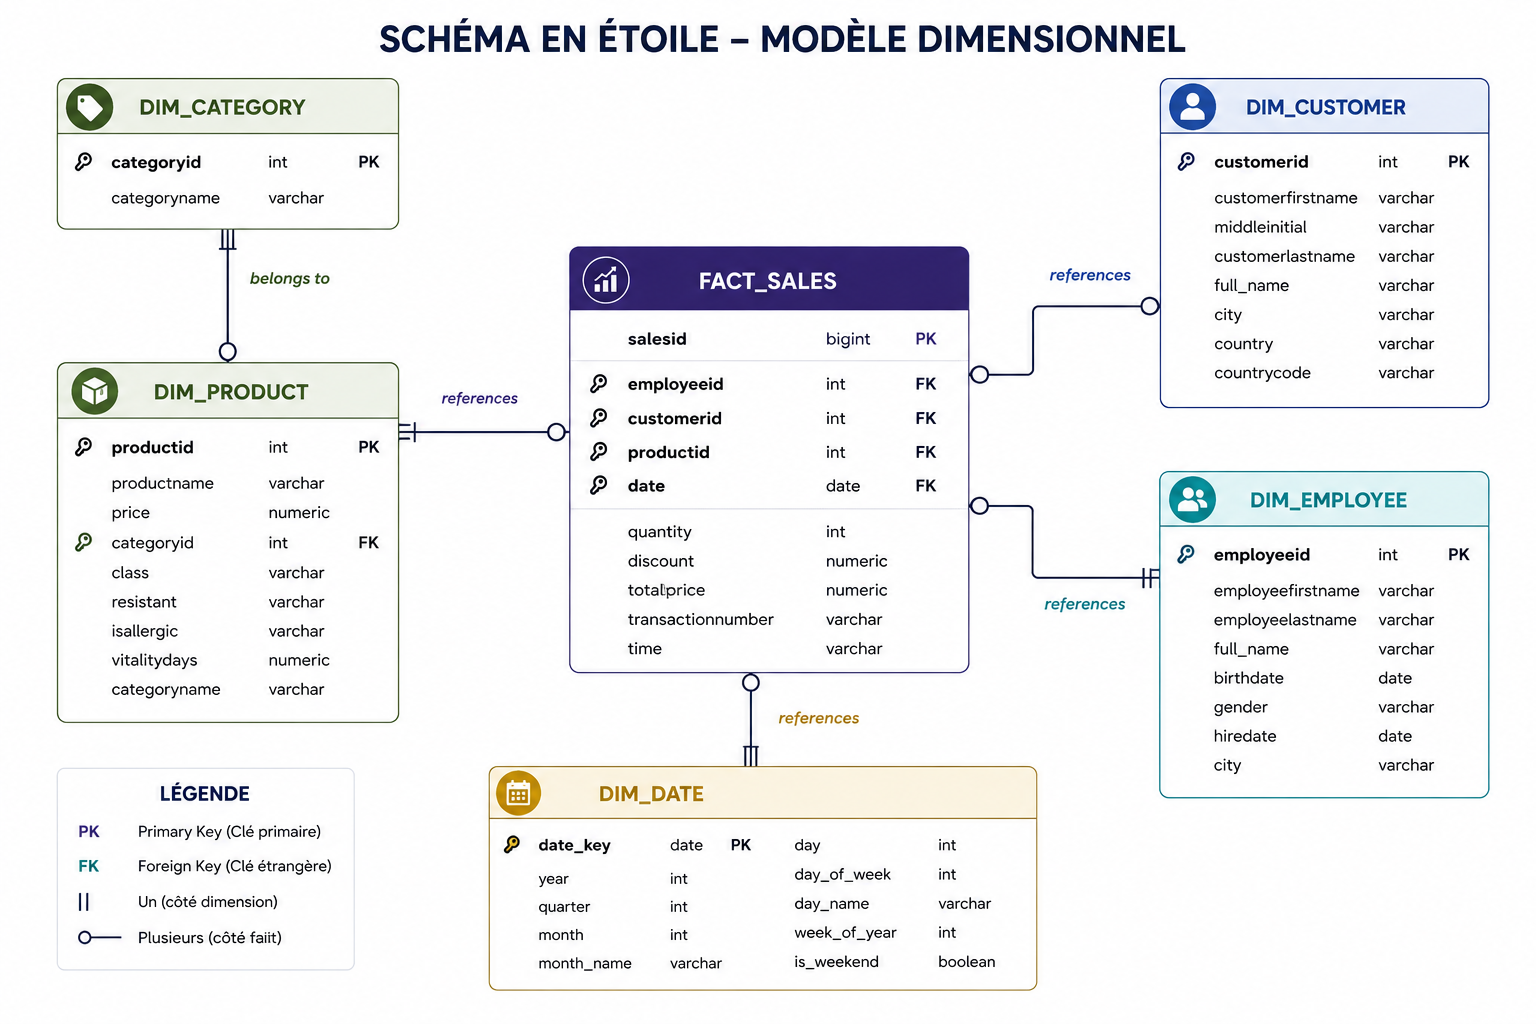
\includegraphics[width=\textwidth,height=8cm,keepaspectratio]{images/data_model.png}
\caption{Le schéma en étoile -- Diagramme entité-relation}
\label{fig:data-model}
\end{figure}

\subsection{Vues matérialisées et index}

Pour optimiser les performances des requêtes du tableau de bord, cinq vues matérialisées ont été créées :

\begin{table}[H]
\centering
\rowcolors{2}{LightGray}{white}
\begin{tabularx}{\textwidth}{>{\bfseries}p{3.5cm}X}
\toprule
\rowcolor{TableHeader}
\color{white}Vue & \color{white}Objectif \\
\midrule
\texttt{mv\_daily\_sales} & Agrégations quotidiennes pour les KPIs et séries temporelles. \\
\texttt{mv\_monthly\_sales} & Tendances mensuelles et comparaisons annuelles. \\
\texttt{mv\_customer\_segmentation} & Segmentation client (VIP, Régulier, Occasionnel, Nouveau). \\
\texttt{mv\_top\_products} & Classement des produits par chiffre d'affaires et volume. \\
\texttt{mv\_employee\_performance} & Métriques de performance individuelle des employés. \\
\bottomrule
\end{tabularx}
\caption{Vues matérialisées du schéma en étoile}
\label{tab:materialized-views}
\end{table}

Des index composites et fonctionnels ont été ajoutés pour accélérer les requêtes les plus fréquentes, notamment sur les colonnes de date, de produit et de transaction.

\section{Le Pipeline ETL en Python}

\subsection{Objectif du pipeline}

Le pipeline ETL constitue le moteur d'alimentation de notre architecture. Son objectif est de transformer les fichiers CSV sources en un schéma en étoile structuré et indexé sous PostgreSQL. Contrairement à une approche avec un outil dédié comme Apache Hop, le pipeline a été entièrement développé en Python avec les bibliothèques \texttt{pandas} et \texttt{SQLAlchemy}.

Le flux respecte le triptyque décisionnel standard et s'articule autour de cinq modules spécialisés :

\begin{center}
\texttt{extractor.py} $\rightarrow$ \texttt{transformer.py} $\rightarrow$ \texttt{validator.py} $\rightarrow$ \texttt{loader.py} $\rightarrow$ \texttt{sync.py}
\end{center}

\begin{quotation}
\noindent\textbf{Choix technique :}\newline
Le choix d'un pipeline Python plutôt qu'un outil ETL visuel permet une intégration plus étroite avec le reste du code, un contrôle fin de chaque étape de transformation, et la possibilité d'automatiser l'ensemble du processus via un simple script.
\end{quotation}

\subsection{Extraction (extractor.py)}

La phase d'extraction lit les fichiers CSV sources à l'aide de \texttt{pandas.read\_csv()}. Sept fichiers sont chargés :

\begin{itemize}
  \item \texttt{categories.csv} (11 lignes) -- Référentiel des catégories ;
  \item \texttt{products.csv} ($\sim$450 lignes) -- Informations produits ;
  \item \texttt{customers.csv} ($\sim$100\,000 lignes) -- Données clients ;
  \item \texttt{employees.csv} ($\sim$50 lignes) -- Données employés ;
  \item \texttt{cities.csv} ($\sim$1\,000 lignes) -- Référentiel des villes ;
  \item \texttt{countries.csv} ($\sim$100 lignes) -- Référentiel des pays ;
  \item \texttt{sales.csv} ($\sim$6\,690\,599 lignes) -- Transactions de vente.
\end{itemize}

Des vérifications sont effectuées : existence du fichier, correspondance du nombre de colonnes et inférence des types de données.

\subsection{Transformation (transformer.py)}

La phase de transformation est la plus riche du pipeline. Elle comprend plusieurs étapes :

\textbf{Nettoyage des dates :} La colonne \texttt{SalesDate} est convertie au format datetime. Les dates invalides sont coercées à \texttt{NaT} et les lignes correspondantes ($\sim$67\,000, soit environ 1\,\%) sont supprimées. La date et l'heure sont ensuite séparées en deux colonnes distinctes.

\textbf{Standardisation des colonnes :} Tous les noms de colonnes sont convertis en \texttt{snake\_case}. Les suffixes de désambiguïsation (\texttt{\_x}, \texttt{\_y}) sont résolus par un renommage explicite.

\textbf{Enrichissement des dimensions :}
\begin{itemize}
  \item \texttt{dim\_product} est enrichie avec le nom de la catégorie via une jointure avec \texttt{categories.csv} ;
  \item \texttt{dim\_customer} est enrichie avec la ville, le pays et le code postal via des jointures avec \texttt{cities.csv} et \texttt{countries.csv} ;
  \item \texttt{dim\_employee} est enrichie avec le nom de la ville via une jointure avec \texttt{cities.csv}.
\end{itemize}

\textbf{Génération de la dimension date :} La table \texttt{dim\_date} est générée programmatiquement à partir de l'intervalle des dates de vente. Les colonnes dérivées incluent : année, mois, trimestre, jour de semaine, nom du mois, indicateur de week-end, etc.

\textbf{Nettoyage des faits :} Le prix total (\texttt{totalprice}) est calculé comme \texttt{quantity $\times$ price} pour corriger les valeurs nulles dans la source.

\subsection{Validation (validator.py)}

Un moteur de validation vérifie l'intégrité des données avant le chargement :

\begin{itemize}
  \item Contrôle d'unicité des clés primaires (HIGH) ;
  \item Vérification des contraintes NOT NULL (HIGH) ;
  \item Validation des valeurs positives pour \texttt{quantity}, \texttt{totalprice}, \texttt{discount} (HIGH) ;
  \item Vérification de l'intégrité référentielle des clés étrangères (HIGH) ;
  \item Contrôle du nombre de colonnes (MEDIUM).
\end{itemize}

Le pipeline est bloqué si une règle de sévérité HIGH échoue.

\subsection{Chargement (loader.py)}

La phase de chargement insère les données dans PostgreSQL en respectant l'ordre des dépendances de clés étrangères :

\begin{enumerate}
  \item \texttt{dim\_category} (aucune dépendance) ;
  \item \texttt{dim\_product} (dépend de \texttt{dim\_category}) ;
  \item \texttt{dim\_customer} (aucune dépendance) ;
  \item \texttt{dim\_employee} (aucune dépendance) ;
  \item \texttt{dim\_date} (aucune dépendance) ;
  \item \texttt{fact\_sales} (dépend de toutes les dimensions).
\end{enumerate}

Pour les dimensions (moins de 100\,000 lignes), la méthode \texttt{method="multi"} est utilisée. Pour la table de faits ($\sim$6,7 millions de lignes), un chargement par lots de 5\,000 lignes est effectué pour rester sous la limite des paramètres PostgreSQL (65\,535).

\begin{resultbox}{Performance du chargement}
Le chargement complet des $\sim$6,7 millions de lignes de \texttt{fact\_sales} s'effectue en 10 à 20 minutes avec la méthode \texttt{multi-row INSERT}, offrant un bon compromis entre simplicité et performance.
\end{resultbox}

\subsection{Synchronisation et vérification (sync.py)}

Après le chargement, un module de synchronisation vérifie :
\begin{itemize}
  \item l'existence de toutes les tables ;
  \item le comptage des lignes ;
  \item l'intégrité des clés étrangères ;
  \item la détection de dérive de schéma.
\end{itemize}

Les vues matérialisées sont ensuite rafraîchies avant la mise à disposition des données.

\section{Architecture de l'API REST}

\subsection{Présentation générale}

L'API est construite avec \textbf{FastAPI}, un framework Python moderne pour la construction d'APIs REST. Elle suit une architecture multicouche avec une séparation claire des responsabilités :

\begin{figure}[H]
\centering
\includegraphics[width=\textwidth,height=8cm,keepaspectratio]{images/sequence_diagram.png}
\caption{Diagramme de séquence -- Chargement d'une page du tableau de bord}
\label{fig:sequence-diagram}
\end{figure}

\subsection{Organisation en couches}

L'API est organisée selon le principe de séparation des préoccupations (\textit{Separation of Concerns}) :

\begin{itemize}
  \item \textbf{Couche API (routeurs) :} expose les endpoints REST et gère les paramètres de requête. Située dans \texttt{app/api/}, elle contient huit routeurs : \texttt{dashboard}, \texttt{sales}, \texttt{products}, \texttt{customers}, \texttt{employees}, \texttt{basket}, \texttt{filters}, \texttt{insights}.
  \item \textbf{Couche service :} contient la logique métier. Chaque service orchestre les appels au repository et construit les objets de réponse (\texttt{dashboard\_service.py}, \texttt{product\_service.py}, etc.).
  \item \textbf{Couche repository :} un repository unique (\texttt{DashboardRepository}) centralise toutes les requêtes SQLAlchemy, évitant la duplication des accès à la base de données.
  \item \textbf{Couche modèle (ORM) :} définit les modèles SQLAlchemy correspondant au schéma en étoile (\texttt{dim\_category.py}, \texttt{dim\_product.py}, \texttt{dim\_customer.py}, \texttt{dim\_employee.py}, \texttt{dim\_date.py}, \texttt{fact\_sales.py}).
  \item \textbf{Couche schéma (Pydantic) :} définit les modèles de validation et de sérialisation avec Pydantic, générant automatiquement la documentation OpenAPI.
\end{itemize}

\begin{table}[H]
\centering
\rowcolors{2}{LightGray}{white}
\begin{tabularx}{\textwidth}{>{\bfseries}p{3cm}X}
\toprule
\rowcolor{TableHeader}
\color{white}Principe & \color{white}Application \\
\midrule
Séparation des responsabilités & Chaque couche a un rôle unique. \\
Injection de dépendances & Sessions DB injectées via \texttt{Depends()}. \\
Cache mémoire & Décorateur de cache pour les requêtes coûteuses. \\
Vues matérialisées & Agrégations pré-calculées pour des réponses instantanées. \\
Validation Pydantic & Schémas stricts avec documentation automatique. \\
\bottomrule
\end{tabularx}
\caption{Principes de conception de l'API}
\label{tab:api-principles}
\end{table}

\subsection{Endpoints principaux}

L'API expose les endpoints suivants :

\begin{longtable}{>{\ttfamily}p{4.5cm}>{\bfseries}p{1.5cm}p{6.5cm}}
\caption{Principaux endpoints de l'API REST}
\label{tab:api-endpoints}
\endfirsthead
\toprule
\rowcolor{TableHeader}
\color{white}Endpoint & \color{white}Méthode & \color{white}Description \\
\midrule
\endhead
\bottomrule
\endfoot
\toprule
\rowcolor{TableHeader}
\color{white}Endpoint & \color{white}Méthode & \color{white}Description \\
\midrule
/api/dashboard/summary & GET & KPIs principaux (CA, quantités, transactions, panier moyen). \\
/api/sales/over-time & GET & Évolution mensuelle du chiffre d'affaires. \\
/api/sales/by-category & GET & Répartition du CA par catégorie. \\
/api/sales/by-city & GET & Distribution géographique des ventes. \\
/api/products/all & GET & Liste des produits avec performances. \\
/api/products/price-distribution & GET & Distribution des prix. \\
/api/products/price-volume-matrix & GET & Matrice prix-volume. \\
/api/customers/segments & GET & Segments client (VIP, Régulier, etc.). \\
/api/customers/top & GET & Meilleurs clients. \\
/api/employees/top & GET & Classement des employés. \\
/api/employees/performance-by-age & GET & Performance par tranche d'âge. \\
/api/basket/analysis & GET & Analyse du panier (règles d'association). \\
/api/insights/revenue-concentration & GET & Concentration du chiffre d'affaires. \\
/api/insights/month-over-month & GET & Croissance mensuelle. \\
/api/insights/customer-rfm & GET & Segmentation RFM. \\
/api/filters/ & GET & Options de filtrage (dates, catégories, etc.). \\
\end{longtable}

\begin{quotation}
\noindent\textbf{Architecture REST :}\newline
Tous les endpoints sont accessibles via HTTP GET et retournent des réponses JSON. Les paramètres de filtrage (dates, catégories, seuils) sont passés en paramètres de requête. L'API est documentée automatiquement via Swagger à l'adresse \texttt{/api/docs}.
\end{quotation}

\chapter{Tableaux de bord web (Dashboard interactif)}

\section{Objectif général}

La couche de présentation du projet consiste en un tableau de bord web interactif qui consomme l'API REST FastAPI pour afficher les indicateurs de performance. Développé avec \textbf{Next.js 14} (App Router), \textbf{TypeScript} et \textbf{Recharts}, il offre une expérience utilisateur moderne, réactive et entièrement navigable.

L'objectif principal du tableau de bord est de fournir une vision synthétique et dynamique de l'activité commerciale. Les utilisateurs peuvent analyser les performances globales, suivre l'évolution des ventes, comparer les produits, étudier le comportement des clients, mesurer la contribution des employés et explorer les associations entre produits.

L'interface est organisée autour de cinq pages thématiques, accessibles via une barre de navigation latérale :

\begin{itemize}
  \item une page dédiée à la performance des ventes (page d'accueil) ;
  \item une page consacrée à l'analyse des produits ;
  \item une page centrée sur le comportement des clients ;
  \item une page dédiée à la performance des employés ;
  \item une page d'analyse du panier basée sur les règles d'association.
\end{itemize}

Chaque page regroupe des indicateurs clés de performance (KPI), des graphiques analytiques et des filtres interactifs permettant d'explorer les données selon différents axes : plage de dates, catégorie, ville ou seuils de lift.

\begin{table}[H]
\centering
\rowcolors{2}{LightGray}{white}
\begin{tabularx}{\textwidth}{>{\bfseries}p{3cm}X}
\toprule
\rowcolor{TableHeader}
\color{white}Technologie & \color{white}Rôle \\
\midrule
Next.js 14 (App Router) & Framework React avec routage par fichiers. \\
TypeScript & Typage statique sur l'ensemble du code. \\
React 18 & Bibliothèque de composants UI. \\
Tailwind CSS & Framework CSS utilitaire. \\
Recharts & Bibliothèque de graphiques React. \\
TanStack React Query & Gestion d'état serveur, cache et rechargement automatique. \\
shadcn/ui & Primitives UI accessibles et personnalisables. \\
Lucide React & Bibliothèque d'icônes. \\
date-fns & Manipulation et formatage des dates. \\
\bottomrule
\end{tabularx}
\caption{Stack technologique du frontend}
\label{tab:frontend-stack}
\end{table}

\section{Page ventes (Accueil)}

La page des ventes constitue la vue principale du tableau de bord. Elle fournit une vision globale de la performance commerciale de l'entreprise à travers les indicateurs les plus importants.

\begin{figure}[H]
\centering
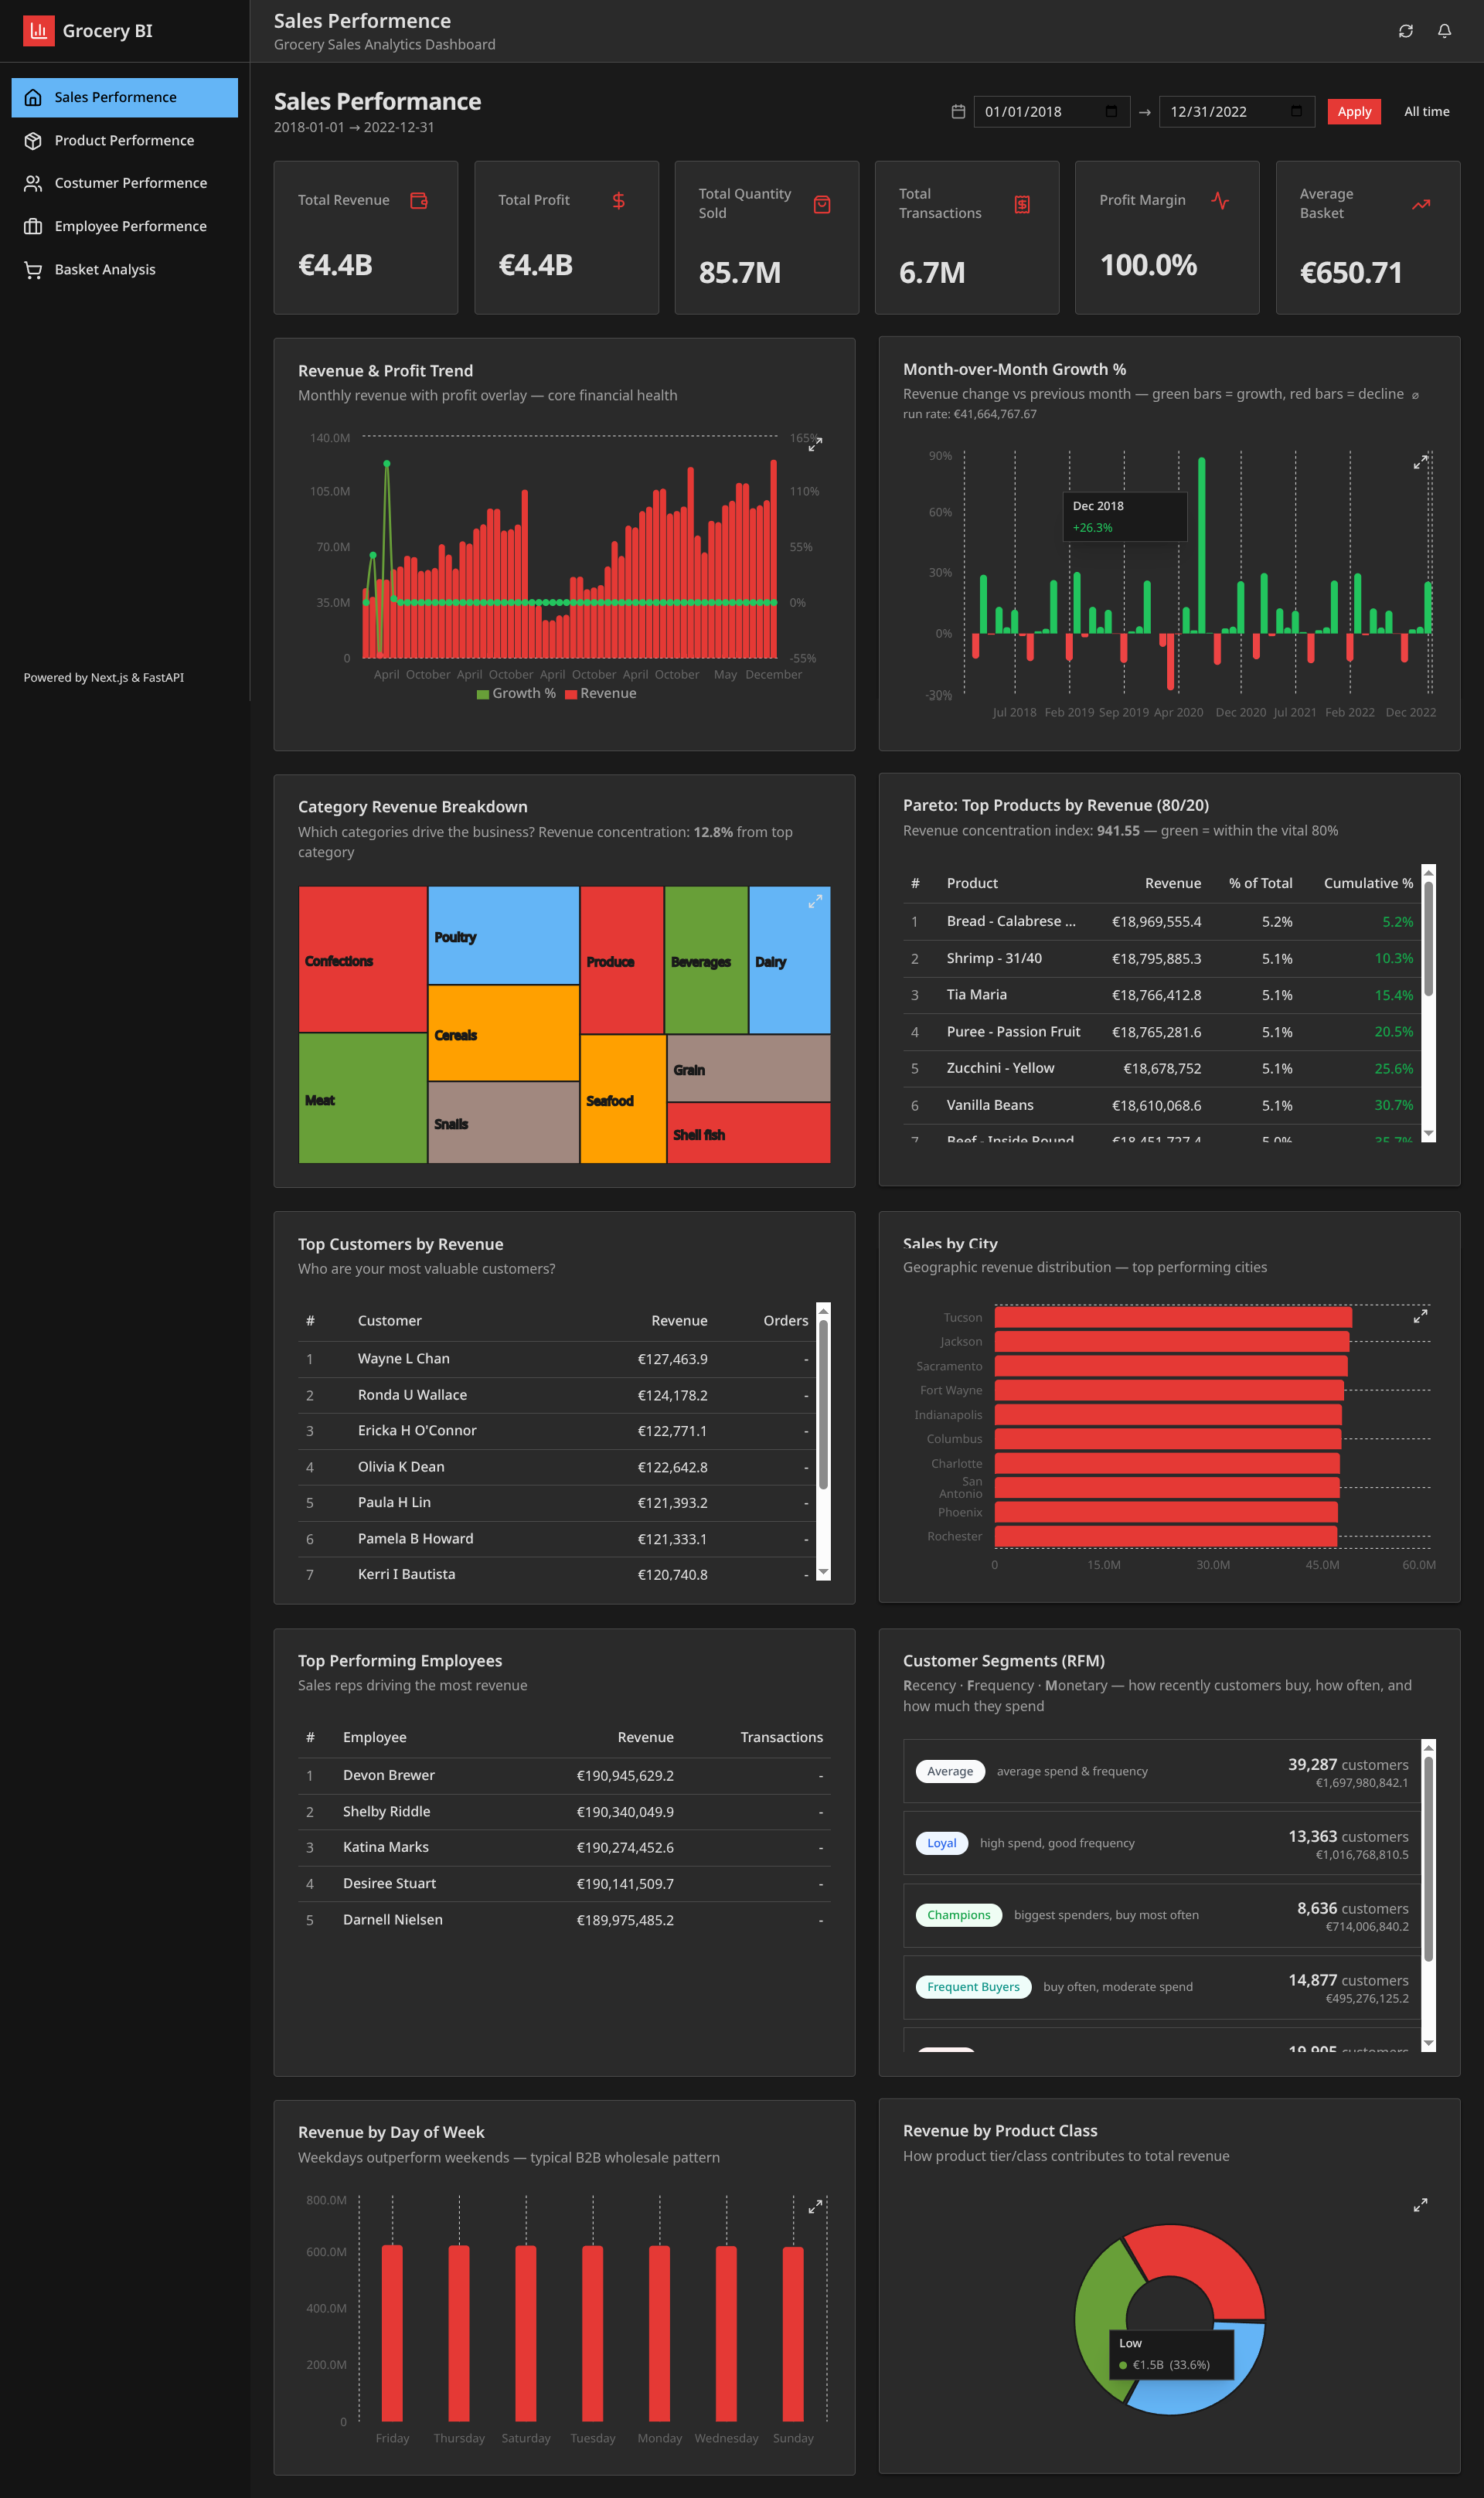
\includegraphics[width=\textwidth,height=8cm,keepaspectratio]{images/sale_performance.png}
\caption{Tableau de bord d'analyse des ventes -- Page d'accueil}
\label{fig:sales-performance}
\end{figure}

\subsection{Indicateurs clés (KPIs)}

La première ligne affiche six indicateurs synthétiques :

\begin{table}[H]
\centering
\rowcolors{2}{LightGray}{white}
\begin{tabularx}{\textwidth}{>{\bfseries}p{3.5cm}p{2.5cm}X}
\toprule
\rowcolor{TableHeader}
\color{white}KPI & \color{white}Format & \color{white}Source API \\
\midrule
Chiffre d'affaires total & Monétaire (€) & \texttt{dashboard/summary} \\
Profit total & Monétaire (€) & \texttt{insights/growth-metrics} \\
Quantité totale vendue & Nombre & \texttt{dashboard/summary} \\
Nombre de transactions & Nombre & \texttt{dashboard/summary} \\
Marge bénéficiaire & Pourcentage & \texttt{insights/growth-metrics} \\
Panier moyen & Monétaire (€) & \texttt{dashboard/summary} \\
\bottomrule
\end{tabularx}
\caption{Indicateurs clés de la page ventes}
\label{tab:sales-kpis}
\end{table}

\subsection{Graphiques analytiques}

La page ventes comprend plusieurs visualisations organisées sur deux à trois lignes :

\textbf{Tendance du chiffre d'affaires :} Un graphique combiné (barres + ligne) présente l'évolution mensuelle du chiffre d'affaires avec un overlay du taux de croissance. Ce graphique met en évidence la saisonnalité de l'activité et permet d'identifier les périodes de forte ou de faible demande.

\textbf{Croissance mensuelle (MoM) :} Un diagramme en barres colorées (vert pour une croissance positive, rouge pour une croissance négative) affiche le taux d'évolution d'un mois sur l'autre.

\textbf{Répartition par catégorie :} Un graphique en arborescence (treemap) représente la distribution du chiffre d'affaires par catégorie de produits. La taille de chaque rectangle est proportionnelle au chiffre d'affaires, permettant une lecture rapide des catégories les plus performantes.

\textbf{Analyse de Pareto :} Un tableau classe les produits par contribution au chiffre d'affaires, permettant d'identifier les quelques produits qui génèrent l'essentiel des revenus (principe des 80/20).

Cette page répond donc à plusieurs questions décisionnelles essentielles : quelle est la performance globale de l'entreprise ? Quels mois génèrent le plus de ventes ? Quelles catégories contribuent le plus au chiffre d'affaires ?

\section{Page produits}

La page produits est consacrée à l'analyse de la performance des références commercialisées. Elle permet d'étudier le chiffre d'affaires et la quantité vendue selon les catégories et les produits.

\begin{figure}[H]
\centering
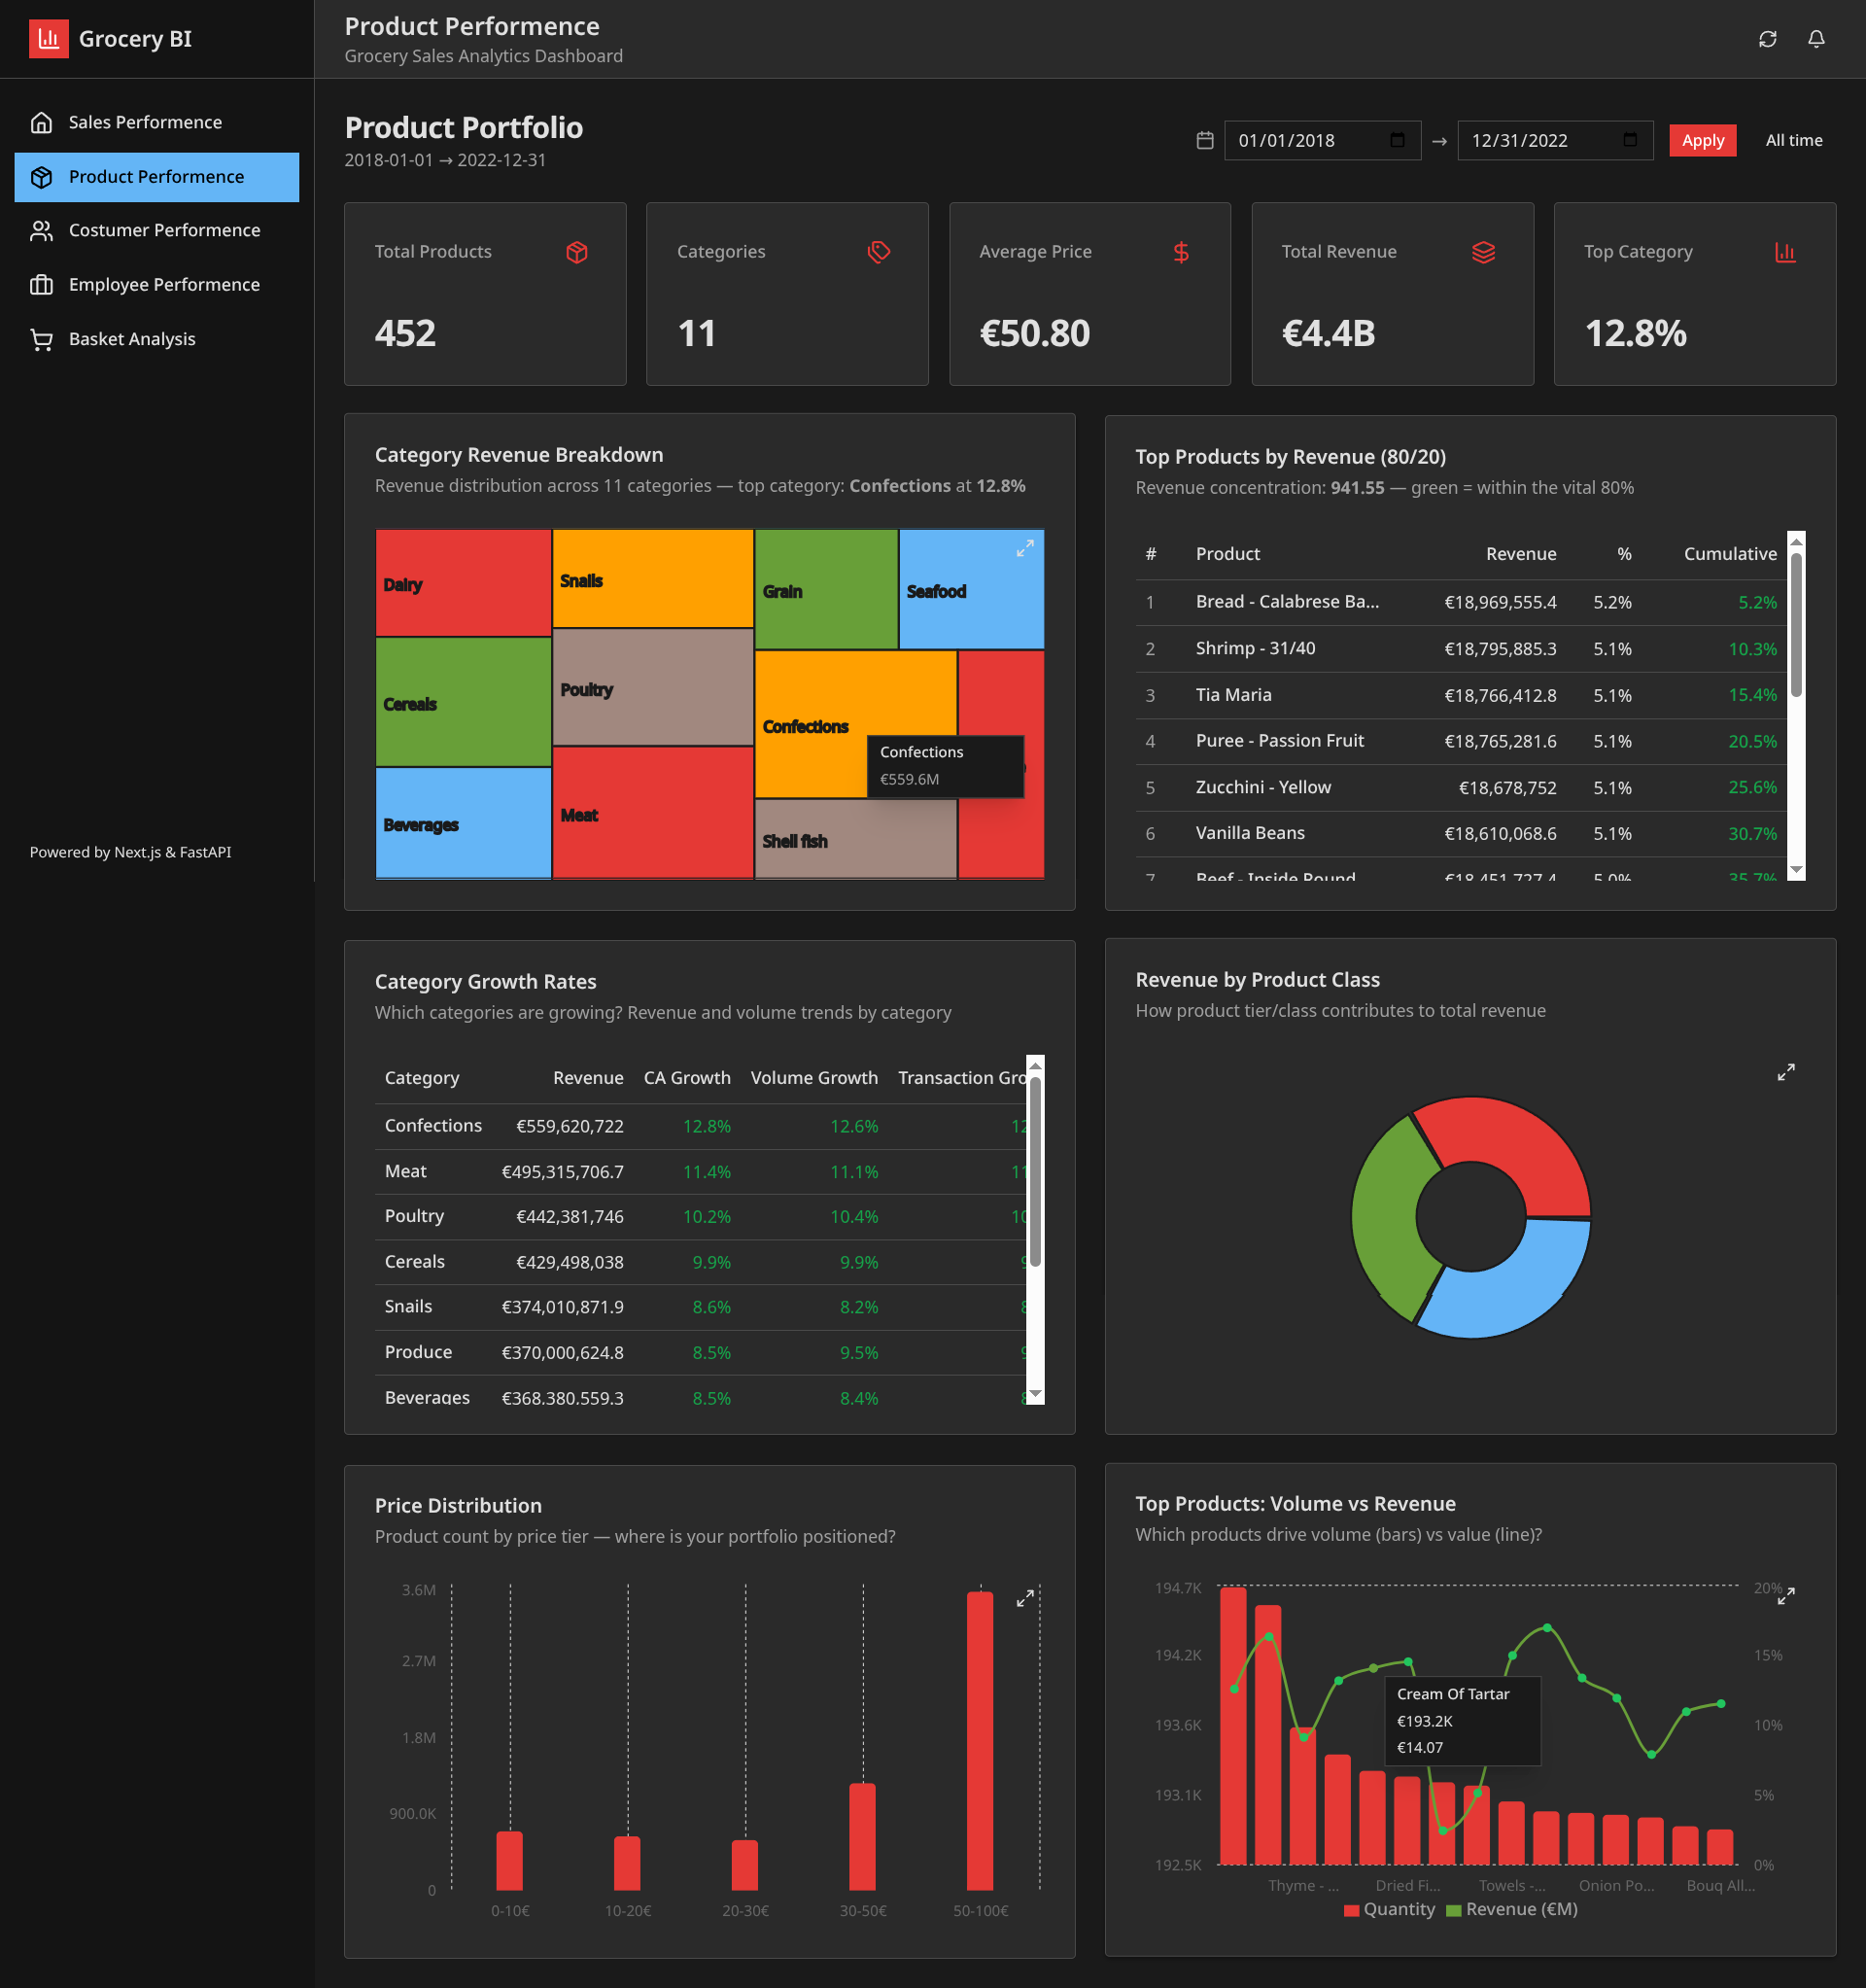
\includegraphics[width=\textwidth,height=8cm,keepaspectratio]{images/product_performance.png}
\caption{Tableau de bord d'analyse des produits}
\label{fig:product-performance}
\end{figure}

La figure \ref{fig:product-performance} présente plusieurs visualisations permettant d'évaluer la contribution des produits au résultat commercial.

\textbf{Distribution des prix :} Un histogramme montre la répartition des prix des produits, permettant d'identifier les gammes de prix les plus représentées dans le catalogue.

\textbf{Matrice prix-volume :} Un nuage de points croise le prix unitaire (axe X) et le volume vendu (axe Y) pour chaque produit. La taille des points peut représenter le chiffre d'affaires. Ce graphique permet d'identifier les produits à fort volume et les produits à forte valeur.

\textbf{Top et flop produits :} Des classements présentent les meilleurs et les moins bons produits selon le chiffre d'affaires et la quantité vendue. Cette comparaison permet de distinguer les produits à forte rotation des produits à faible contribution.

\textbf{Analyse par attributs :} La page explore également l'impact des caractéristiques produit (\texttt{isallergic}, \texttt{resistant}, \texttt{class}) sur les performances commerciales.

Cette page aide à répondre aux questions suivantes : quelles catégories génèrent le plus de chiffre d'affaires ? Quels produits sont les plus vendus ? Quels produits ont une faible performance ? Comment les caractéristiques des produits influencent-elles les ventes ?

\section{Page clients}

La page clients a pour objectif d'analyser la valeur et le comportement de la clientèle. Elle permet d'étudier le nombre de clients, le nombre de clients actifs, le panier moyen, la fréquence d'achat et le taux de réachat.

\begin{figure}[H]
\centering
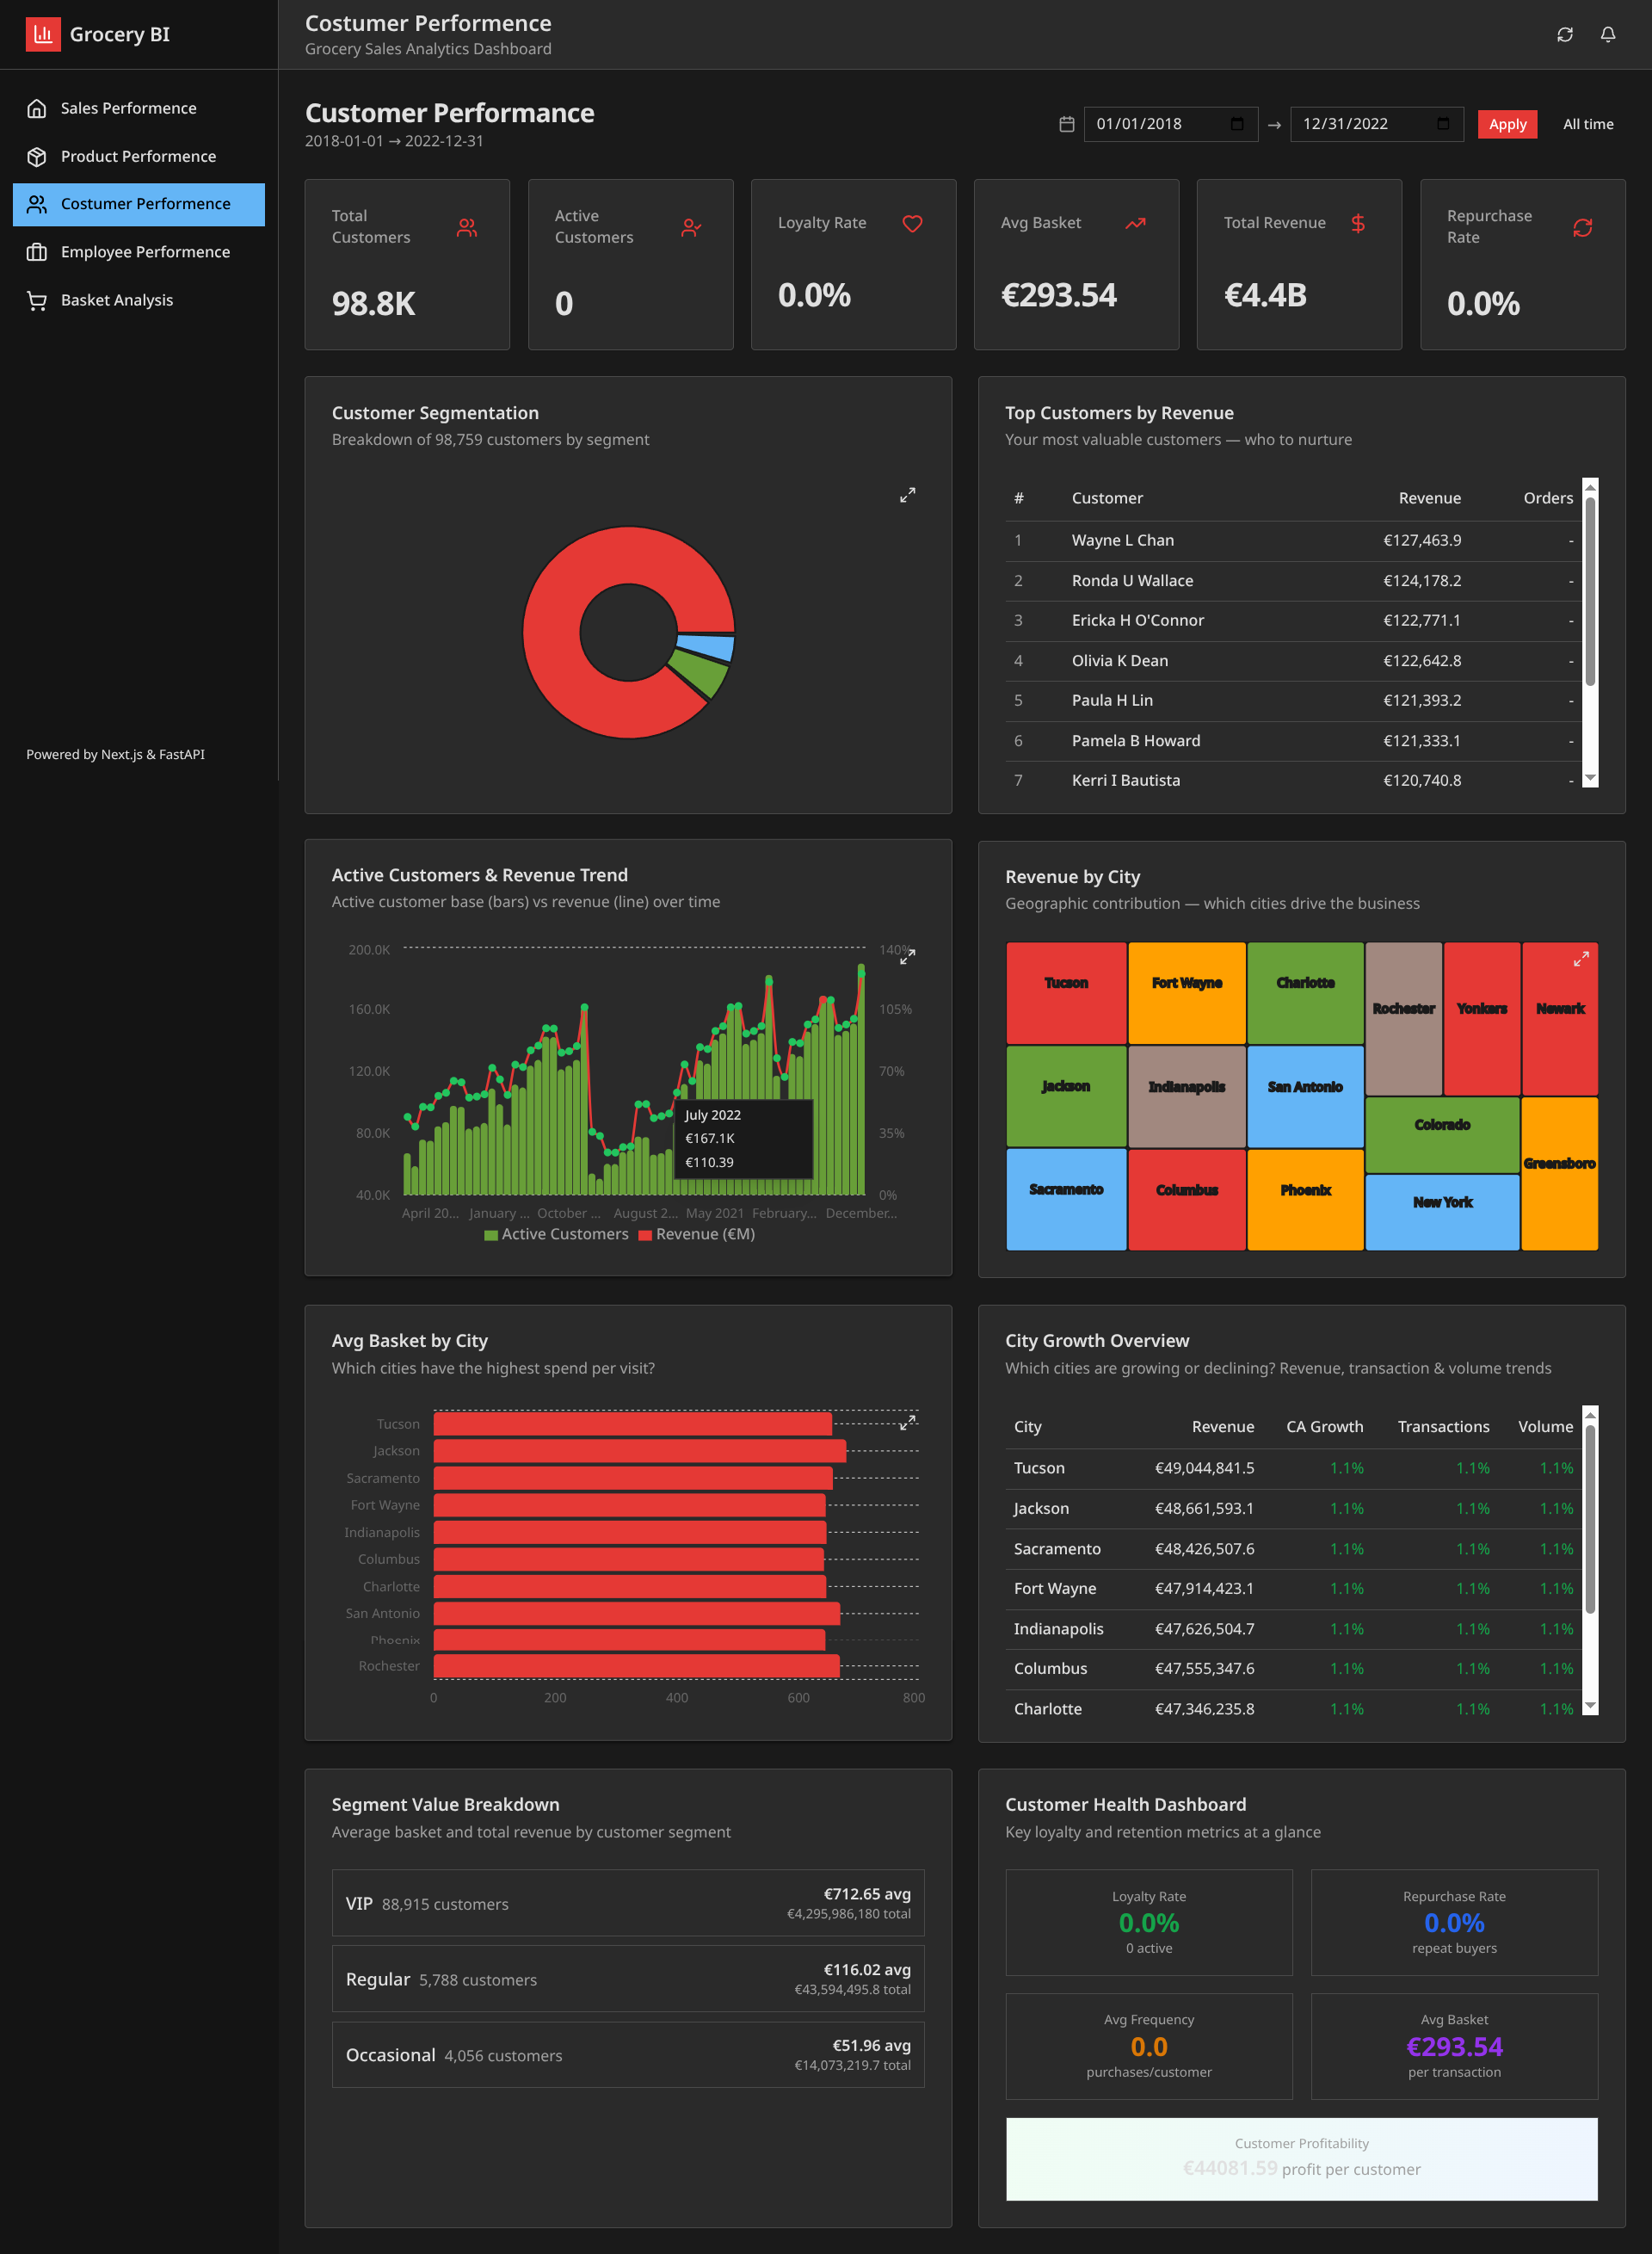
\includegraphics[width=\textwidth,height=8cm,keepaspectratio]{images/customer_performance.png}
\caption{Tableau de bord d'analyse des clients}
\label{fig:customer-performance}
\end{figure}

\textbf{Segmentation RFM :} Une analyse RFM (Récence, Fréquence, Montant) classe les clients en segments : VIP, Régulier, Occasionnel, Nouveau, et Perdu. Cette segmentation est présentée sous forme de diagramme en secteurs ou de tableau.

\textbf{Top clients :} Un classement des clients par chiffre d'affaires permet d'identifier les clients les plus importants.

\textbf{Activité géographique :} Une carte ou un graphique en barres montre la répartition des clients par ville ou par pays. Cette information peut orienter les actions commerciales régionales.

\textbf{PANIER MOYEN PAR VILLE :} L'analyse compare le panier moyen des clients selon leur localisation géographique.

Cette page répond à des questions importantes pour la gestion de la relation client : quels sont les clients les plus actifs ? Quelle est la valeur moyenne d'un client ? Quelles zones géographiques concentrent le plus d'activité ? Quels segments de clientèle méritent une attention particulière ?

\section{Page employés}

La page employés permet d'évaluer la contribution des vendeurs à la performance commerciale globale.

\begin{figure}[H]
\centering
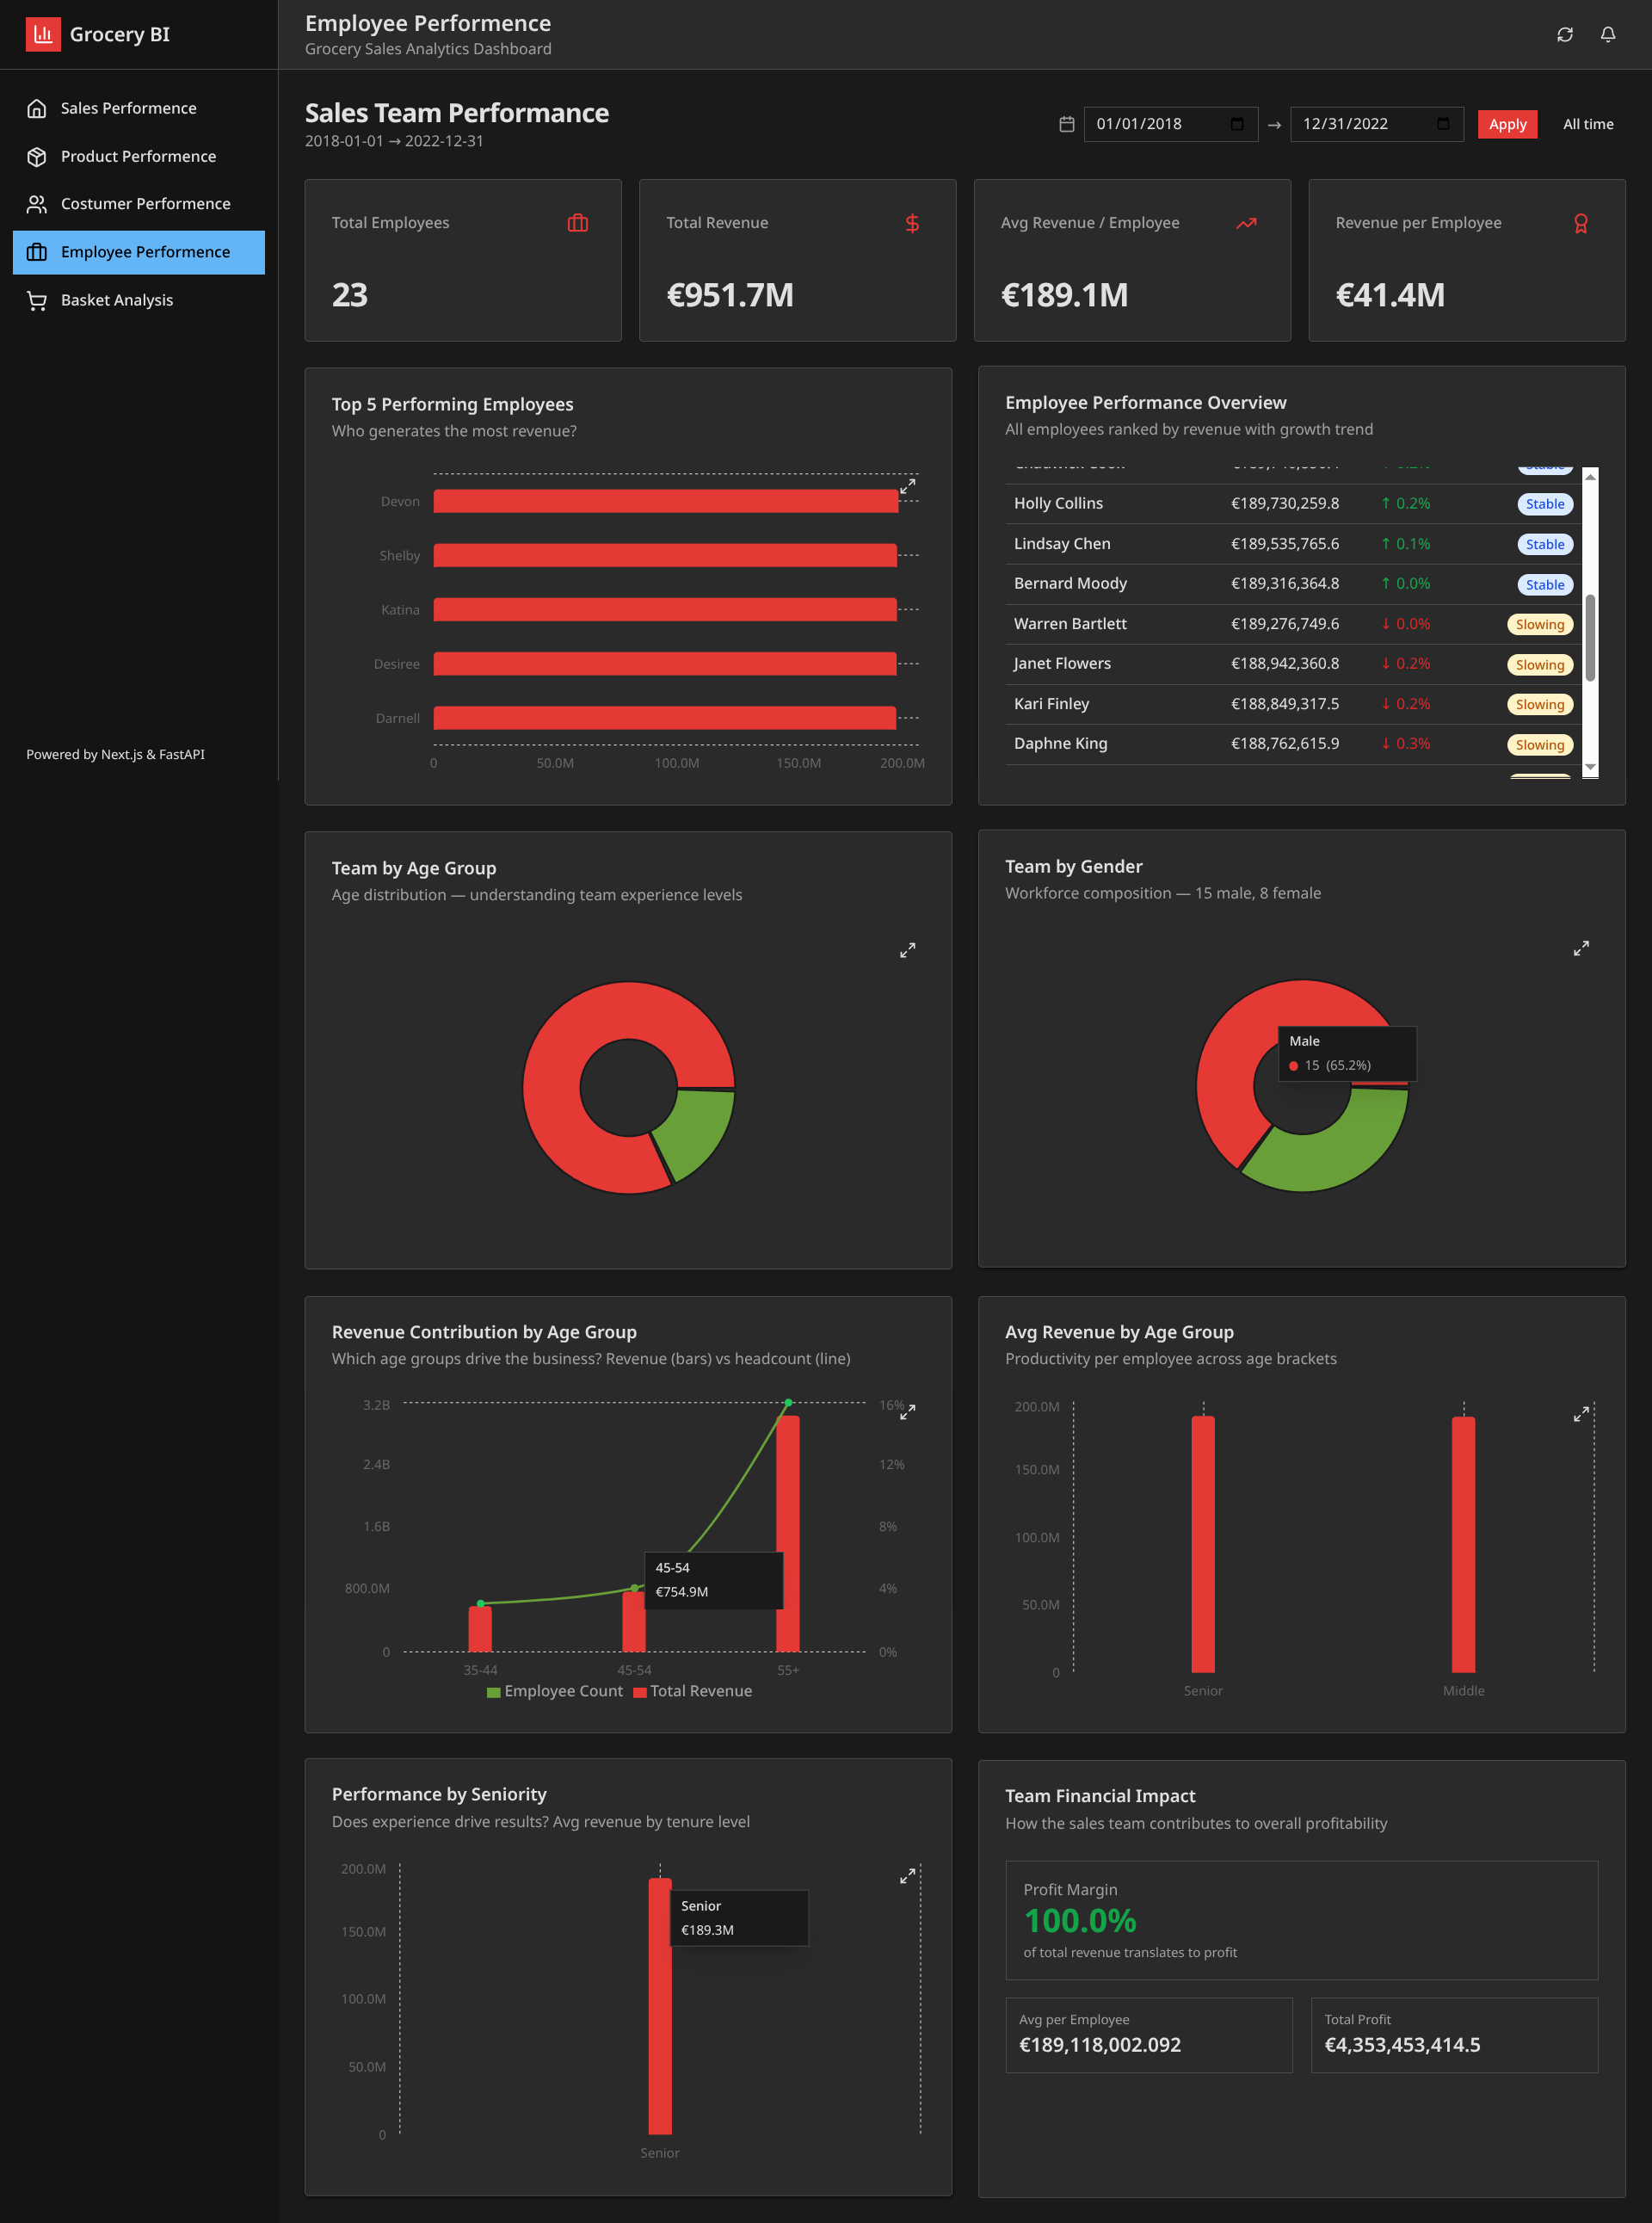
\includegraphics[width=\textwidth,height=8cm,keepaspectratio]{images/employee_performance.png}
\caption{Tableau de bord d'analyse des employés}
\label{fig:employee-performance}
\end{figure}

\textbf{Classement individuel :} Un tableau présente le chiffre d'affaires généré par chaque employé, accompagné du taux de croissance et du nombre de transactions.

\textbf{Performance par tranche d'âge :} Un graphique en barres compare le chiffre d'affaires moyen des employés selon leur tranche d'âge.

\textbf{Performance par ancienneté :} Un graphique analyse la relation entre l'ancienneté des employés et leur performance commerciale.

\textbf{Répartition par genre :} Un diagramme en secteurs montre la distribution des employés par genre et leur contribution au chiffre d'affaires.

Cette page permet de répondre aux questions suivantes : quels employés contribuent le plus au chiffre d'affaires ? Comment la performance varie-t-elle selon les profils ? Existe-t-il des écarts significatifs entre les groupes d'employés ?

\section{Page analyse du panier}

La page d'analyse du panier est consacrée aux règles d'association entre produits (Market Basket Analysis). Elle exploite les données pré-calculées de l'analyse du panier pour afficher les associations les plus pertinentes.

\begin{figure}[H]
\centering
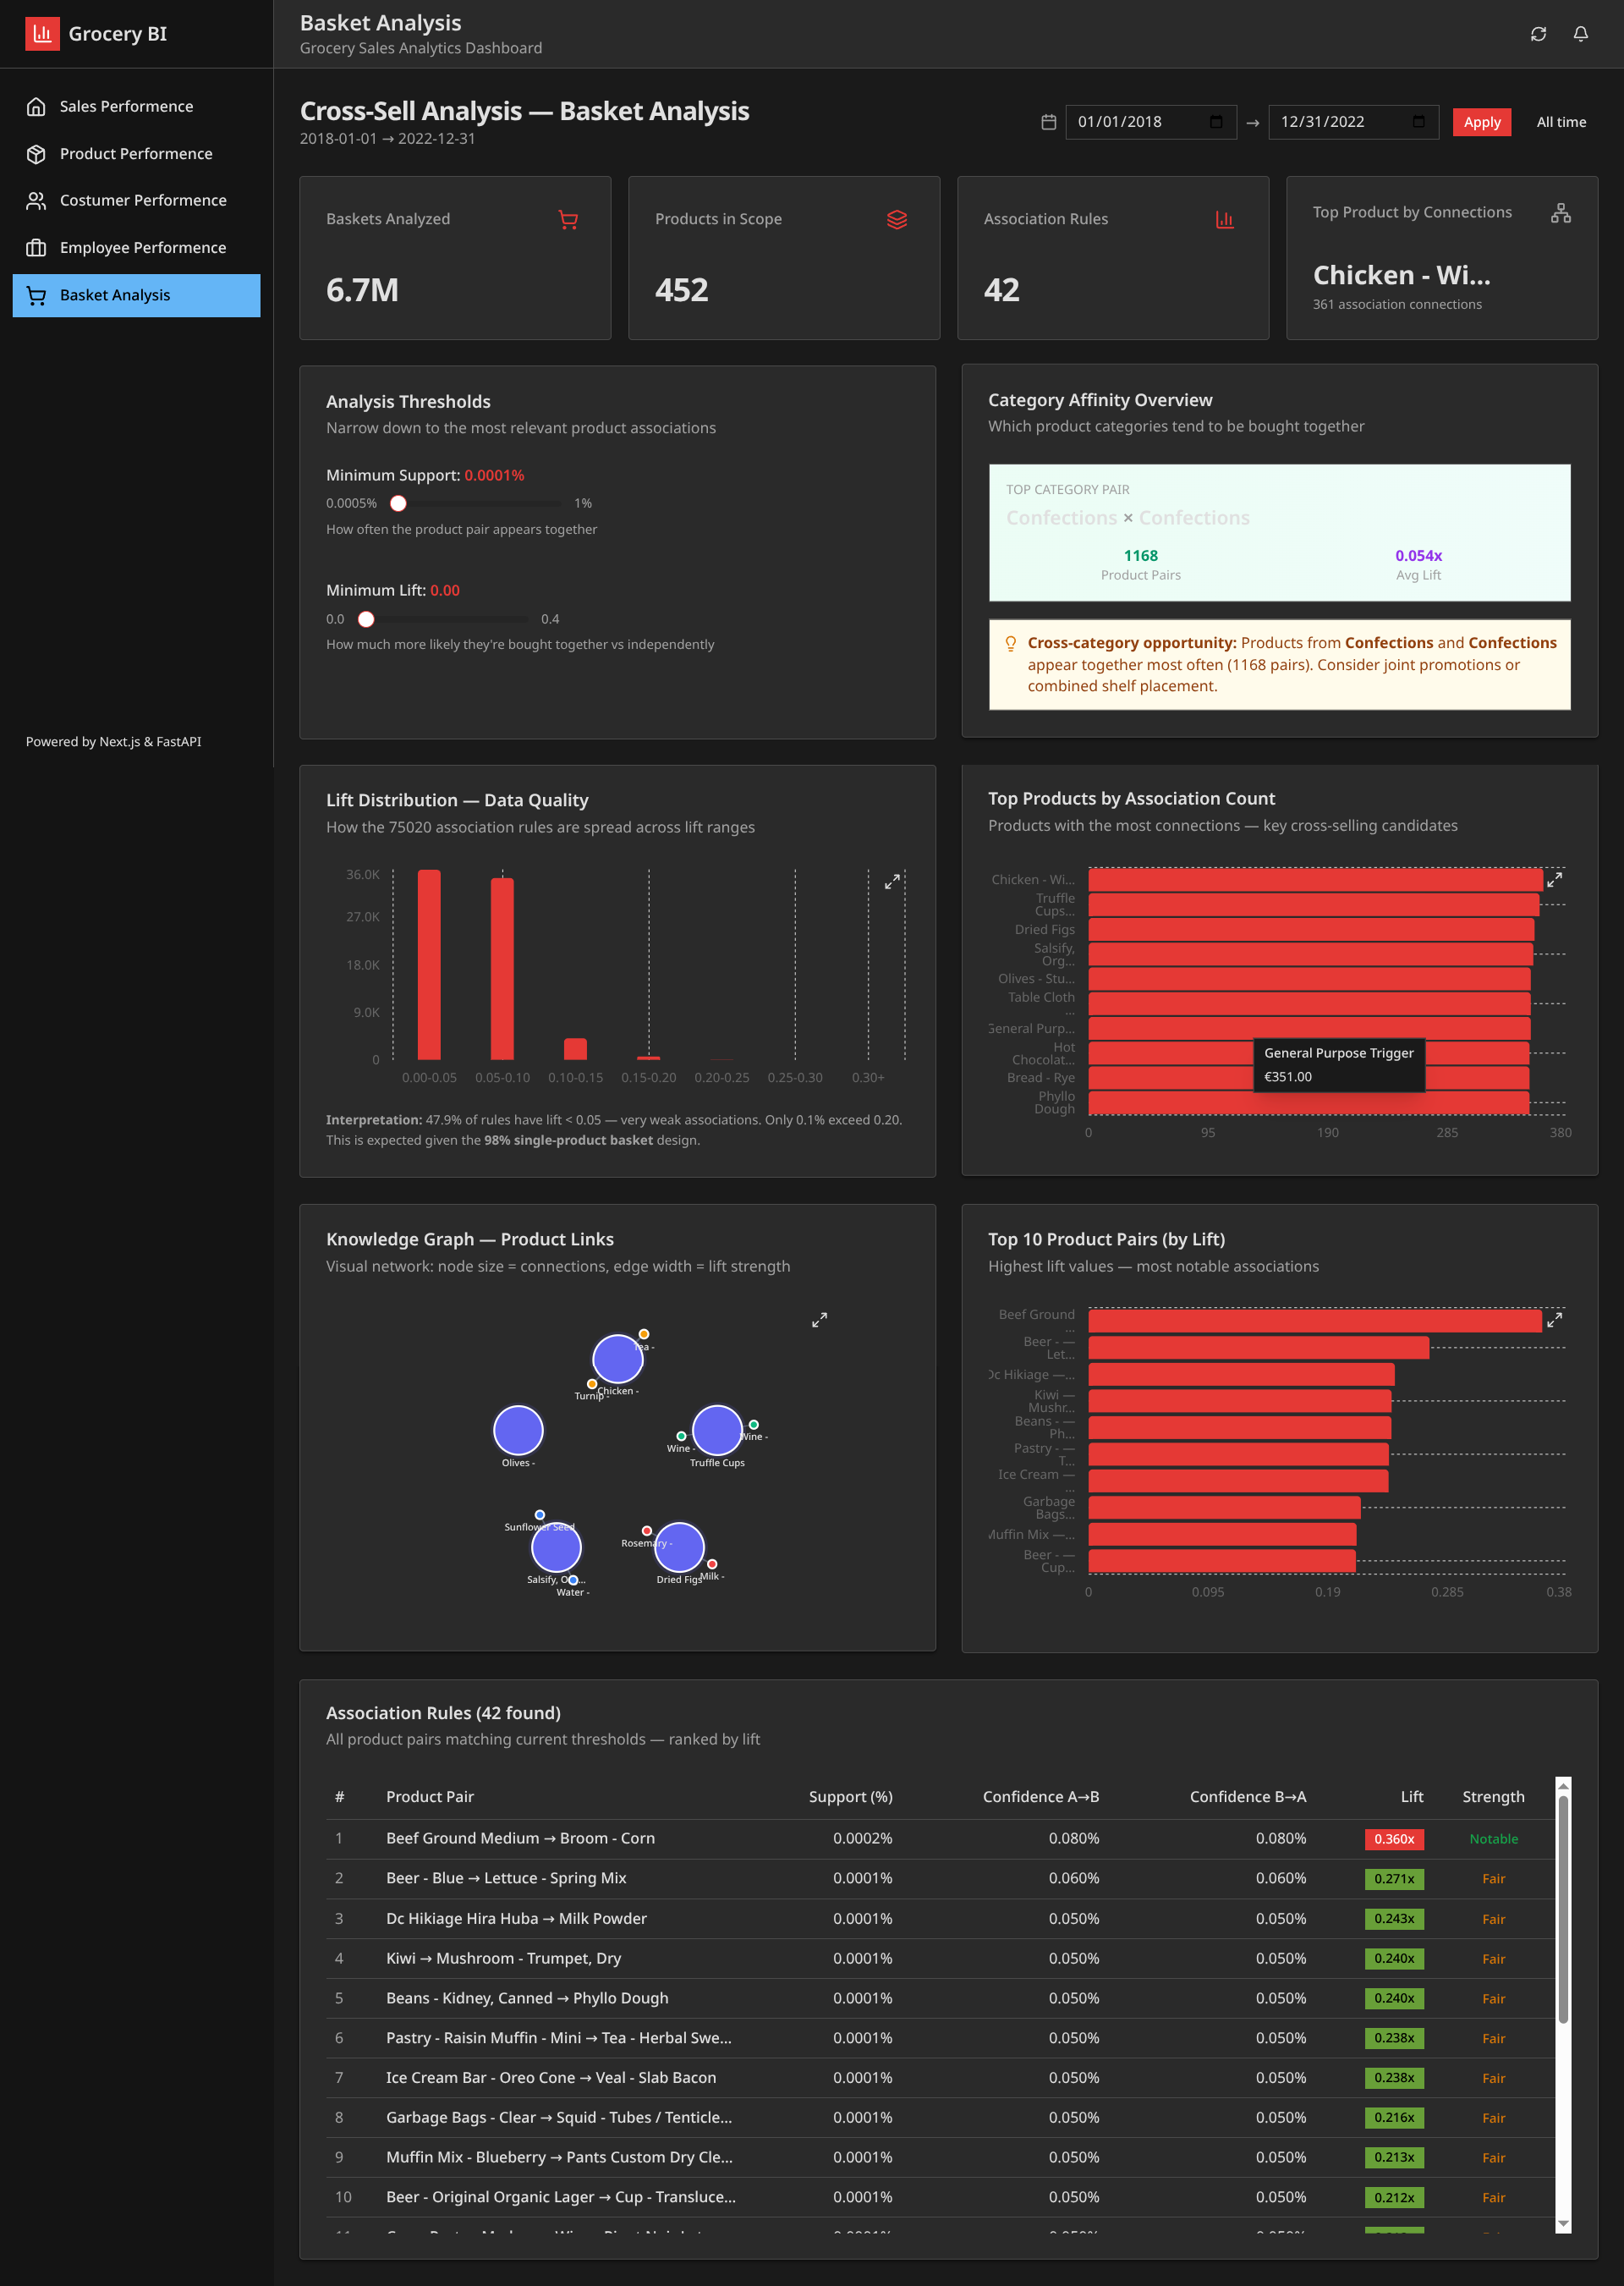
\includegraphics[width=\textwidth,height=8cm,keepaspectratio]{images/basket_analysis.png}
\caption{Tableau de bord d'analyse du panier}
\label{fig:basket-analysis}
\end{figure}

\textbf{Métriques globales :} Nombre total de produits analysés, nombre total de transactions, nombre de règles d'association.

\textbf{Nuage de points (Support vs Lift) :} Chaque point représente une paire de produits. L'axe X représente le lift et l'axe Y le support. Les associations les plus intéressantes se situent dans le quadrant supérieur droit.

\textbf{Produits hubs :} Classement des produits ayant le plus grand nombre de connexions significatives avec d'autres produits.

\textbf{Distribution du lift :} Histogramme montrant la répartition des valeurs de lift sur l'ensemble des règles.

\textbf{Affinités par catégorie :} Tableau des associations entre catégories de produits, avec le lift moyen et le nombre de paires.

\section{Synthèse des apports des tableaux de bord}

Les tableaux de bord web développés dans ce projet couvrent plusieurs niveaux d'analyse. La page ventes fournit une vision globale de la performance commerciale. La page produits permet d'étudier la contribution du catalogue. La page clients apporte une lecture orientée comportement et fidélisation. La page employés permet de suivre la contribution individuelle et collective des vendeurs. Enfin, la page panier ajoute une dimension data mining en révélant les associations entre produits.

L'ensemble de ces pages transforme l'entrepôt de données en un véritable outil d'aide à la décision. Les visualisations ne se limitent pas à présenter les données ; elles permettent d'identifier des tendances, de comparer les performances, de détecter des opportunités commerciales et de soutenir des décisions opérationnelles.

L'architecture technique -- API REST FastAPI couplée à un frontend Next.js avec Recharts -- offre une expérience utilisateur fluide, des temps de réponse rapides grâce aux vues matérialisées et au caching TanStack Query, et une maintenabilité facilitée par la séparation des couches.

\chapter{Data Mining : Analyse du panier}

\section{Introduction}

Dans le cadre de ce projet décisionnel, une étape de \textit{data mining} a été intégrée afin de dépasser la simple visualisation descriptive des indicateurs de vente. L'objectif est d'extraire des connaissances à partir des transactions clients et d'identifier des relations significatives entre les produits achetés ensemble.

La méthode retenue est l'analyse du panier, également appelée \textit{Market Basket Analysis}. Cette technique permet de détecter les associations fréquentes entre les produits au sein des transactions. Elle est largement utilisée dans les systèmes décisionnels commerciaux pour comprendre les comportements d'achat, proposer des recommandations de produits complémentaires et soutenir les actions marketing.

\section{Objectif de l'analyse}

L'objectif principal de l'analyse du panier est de répondre à la question suivante :

\begin{center}
\textit{Quels produits sont fréquemment achetés ensemble dans une même transaction ?}
\end{center}

Cette analyse permet d'identifier des combinaisons de produits présentant un intérêt commercial. Lorsqu'une association forte est détectée entre deux produits, elle peut être utilisée pour recommander un produit complémentaire, créer une offre groupée ou améliorer l'organisation des produits.

Les résultats de cette analyse peuvent être exploités pour :
\begin{itemize}
  \item recommander des produits complémentaires aux clients ;
  \item créer des promotions ou des offres groupées ;
  \item améliorer l'organisation des produits dans les rayons ;
  \item cibler les campagnes marketing ;
  \item augmenter le panier moyen et la valeur des transactions.
\end{itemize}

\begin{resultbox}{Apport du data mining}
L'analyse du panier transforme les données transactionnelles en règles d'association exploitables. Elle permet donc de passer d'une analyse descriptive des ventes à une analyse plus avancée du comportement d'achat.
\end{resultbox}

\section{Données utilisées}

L'analyse repose sur une table transactionnelle appelée \texttt{DF\_Basket}. Cette table représente les produits achetés dans chaque panier. Chaque ligne correspond à un produit appartenant à une transaction donnée.

La structure utilisée pour cette analyse contient principalement :
\begin{itemize}
  \item \texttt{id\_transaction} : l'identifiant unique de la transaction ;
  \item \texttt{productname} : le nom du produit acheté.
\end{itemize}

Ainsi, lorsqu'une transaction contient plusieurs produits, ces produits apparaissent sur plusieurs lignes avec le même identifiant de transaction. Cette organisation permet de comparer les produits entre eux et d'identifier les paires qui apparaissent fréquemment dans les mêmes paniers.

\begin{table}[H]
\centering
\rowcolors{2}{LightGray}{white}
\begin{tabular}{cc}
\toprule
\rowcolor{TableHeader}
\color{white}\textbf{id\_transaction} & \color{white}\textbf{productname} \\
\midrule
1 & whole milk \\
1 & eggs \\
1 & bread \\
2 & whole milk \\
2 & butter \\
3 & coffee \\
3 & sugar \\
\bottomrule
\end{tabular}
\caption{Exemple simplifié de structure transactionnelle utilisée pour l'analyse du panier}
\label{tab:structure-basket}
\end{table}

\section{Principe méthodologique}

La méthodologie adoptée consiste à générer les différentes paires possibles de produits, puis à mesurer la force de l'association entre chaque paire. Afin d'éviter les répétitions, chaque couple de produits est conservé une seule fois.

Par exemple, l'association \textit{bread -- butter} est considérée comme équivalente à \textit{butter -- bread}. Une seule combinaison est donc retenue dans la table d'analyse.

La table finale d'analyse contient les informations suivantes :
\begin{itemize}
  \item le premier produit de la paire ;
  \item le deuxième produit de la paire ;
  \item une colonne d'affichage sous la forme \textit{Produit 1 -- Produit 2} ;
  \item le support de l'association ;
  \item la confidence dans les deux directions ;
  \item le lift de l'association.
\end{itemize}

Cette structure permet ensuite de construire les visualisations dans le tableau de bord web et d'identifier les associations les plus pertinentes d'un point de vue commercial.

\section{Métriques d'association}

Trois métriques principales ont été utilisées pour évaluer la qualité des associations : le support, la confidence et le lift.

\subsection{Support}

Le support mesure la fréquence d'apparition d'une paire de produits dans l'ensemble des transactions.

\[
Support(X,Y) = \frac{\text{Nombre de transactions contenant X et Y}}{\text{Nombre total de transactions}}
\]

Un support élevé signifie que les deux produits apparaissent fréquemment ensemble dans les paniers. Cette métrique permet donc de distinguer les associations courantes des associations rares.

Cependant, le support ne suffit pas à lui seul pour juger la qualité d'une association. Une paire peut avoir un support élevé simplement parce que les deux produits sont très populaires séparément, sans qu'il existe nécessairement une relation forte entre eux.

\subsection{Confidence}

La confidence mesure la probabilité d'acheter un produit sachant qu'un autre produit est déjà présent dans le panier.

\[
Confidence(X \rightarrow Y) = \frac{Support(X,Y)}{Support(X)}
\]

Par exemple, une confidence de 30\,\% pour la règle \textit{X} $\rightarrow$ \textit{Y} signifie que 30\,\% des transactions contenant le produit X contiennent également le produit Y.

Dans ce projet, la confidence est calculée dans les deux directions :
\begin{itemize}
  \item \texttt{Confidence P1} : probabilité d'acheter le produit 2 sachant que le produit 1 est acheté ;
  \item \texttt{Confidence P2} : probabilité d'acheter le produit 1 sachant que le produit 2 est acheté.
\end{itemize}

\subsection{Lift}

Le lift mesure la force réelle de l'association entre deux produits en la comparant à une situation d'indépendance.

\[
Lift(X,Y) = \frac{Support(X,Y)}{Support(X) \times Support(Y)}
\]

Le lift est un indicateur essentiel pour déterminer si deux produits sont réellement associés. Une valeur supérieure à 1 signifie que les deux produits sont achetés ensemble plus souvent que ce que l'on obtiendrait par hasard.

\begin{table}[H]
\centering
\rowcolors{2}{LightGray}{white}
\begin{tabularx}{\textwidth}{>{\bfseries}p{3cm}X}
\toprule
\rowcolor{TableHeader}
\color{white}\textbf{Valeur du lift} & \color{white}\textbf{Interprétation} \\
\midrule
Inférieur à 1 & Association négative : les produits sont moins souvent achetés ensemble que prévu. \\
Égal à 1 & Absence d'association particulière : les produits sont statistiquement indépendants. \\
Entre 1 et 1,5 & Association faible, à interpréter avec prudence. \\
Entre 1,5 et 2 & Association intéressante pour une recommandation croisée. \\
Supérieur à 2 & Association forte, pouvant justifier une offre groupée ou une action marketing ciblée. \\
\bottomrule
\end{tabularx}
\caption{Interprétation de la métrique Lift}
\label{tab:interpretation-lift}
\end{table}

Dans cette analyse, les associations ayant un lift supérieur ou égal à 1,5 sont considérées comme commercialement pertinentes.

\section{Intégration dans le tableau de bord web}

L'analyse du panier a été intégrée dans le tableau de bord web à travers une page spécifique. Cette page permet de visualiser les associations entre les produits et de comparer leurs métriques.

Les principaux éléments affichés sont :
\begin{itemize}
  \item le nombre total de produits analysés ;
  \item le nombre total de transactions ;
  \item un nuage de points représentant les associations selon le support et le lift ;
  \item les produits hubs (ceux avec le plus de connexions) ;
  \item la distribution des valeurs de lift ;
  \item les affinités entre catégories de produits ;
  \item un tableau détaillé contenant les valeurs de support, confidence et lift pour chaque paire.
\end{itemize}

\begin{figure}[H]
\centering
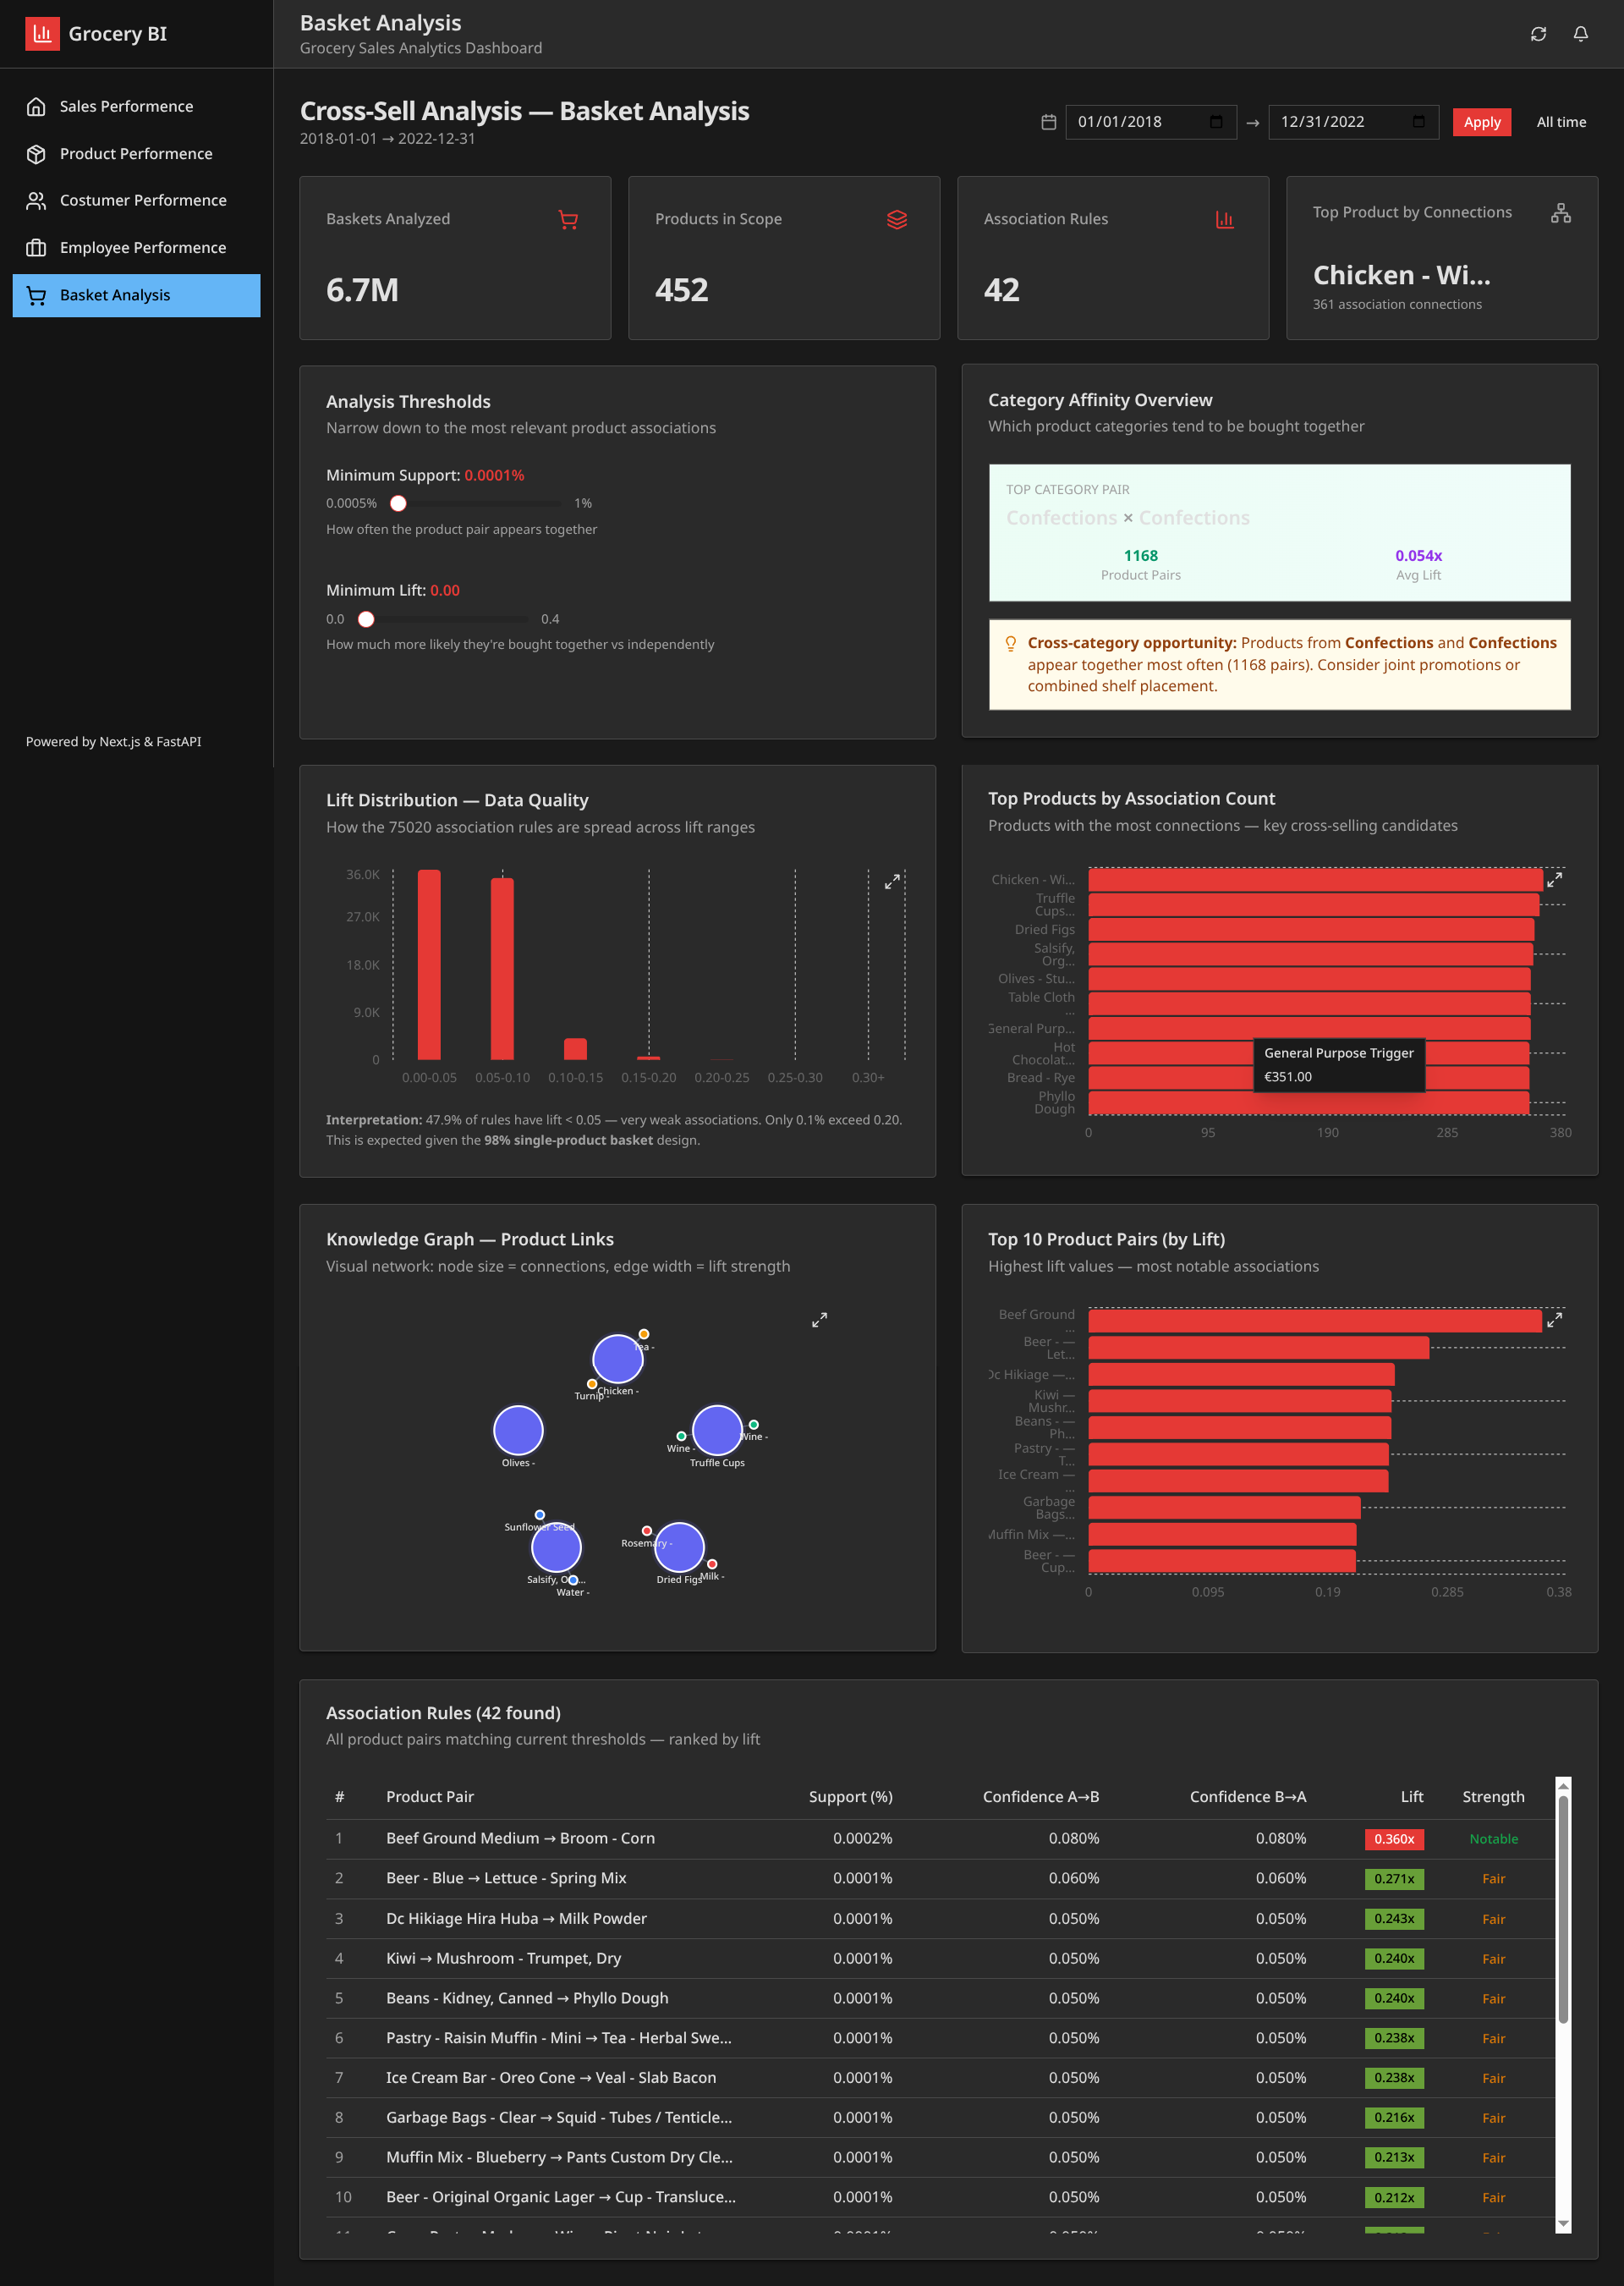
\includegraphics[width=\textwidth,height=8cm,keepaspectratio]{images/basket_analysis.png}
\caption{Page du tableau de bord web dédiée à l'analyse du panier}
\label{fig:basket-analysis-dashboard}
\end{figure}

La figure \ref{fig:basket-analysis-dashboard} présente la page web consacrée à l'analyse du panier. Le nuage de points permet de comparer les associations de produits selon deux dimensions : le support et le lift. Chaque point représente une paire de produits. Les associations situées vers le haut du graphique présentent un support plus élevé, tandis que celles situées vers la droite présentent un lift plus important.

Le tableau détaillé complète cette visualisation en affichant, pour chaque association, les valeurs de support, de confidence dans les deux directions et de lift. Cette représentation facilite l'identification des associations les plus intéressantes pour la recommandation croisée, les offres groupées ou l'optimisation du placement des produits.

\section{Interprétation des résultats}

Les résultats obtenus montrent que certaines associations de produits ressortent de manière significative. Certaines paires présentent un support élevé, ce qui signifie qu'elles apparaissent fréquemment dans les transactions. D'autres présentent un lift élevé, indiquant une relation plus forte que le hasard.

Parmi les associations observées dans le tableau de bord, on retrouve par exemple :
\begin{itemize}
  \item \textit{root vegetables -- other vegetables} ;
  \item \textit{tropical fruit -- citrus fruit} ;
  \item \textit{whipped/sour cream -- berries} ;
  \item \textit{yogurt -- curd} ;
  \item \textit{frozen vegetables -- chicken} ;
  \item \textit{sliced cheese -- sausage}.
\end{itemize}

L'association \textit{root vegetables -- other vegetables} présente un support particulièrement élevé, ce qui montre qu'elle apparaît fréquemment dans les paniers. Cette association peut s'expliquer par la complémentarité naturelle entre différentes catégories de légumes.

D'autres associations, comme \textit{whipped/sour cream -- berries} ou \textit{sliced cheese -- sausage}, présentent un lift élevé. Cela signifie que ces produits sont achetés ensemble plus souvent que prévu dans une situation indépendante. Ces associations sont donc intéressantes pour des recommandations commerciales ciblées.

\section{Exploitation commerciale des résultats}

Les résultats de l'analyse du panier peuvent être transformés en actions commerciales concrètes.

Premièrement, les associations fortes peuvent être utilisées pour recommander des produits complémentaires. Lorsqu'un client achète un produit, le système peut proposer un autre produit fréquemment acheté avec celui-ci.

Deuxièmement, l'entreprise peut créer des offres groupées. Les produits présentant un lift élevé peuvent être regroupés dans des promotions afin d'encourager leur achat simultané.

Troisièmement, les résultats peuvent aider à optimiser l'organisation des rayons. Les produits souvent achetés ensemble peuvent être placés à proximité afin de faciliter l'achat et d'améliorer l'expérience client.

Enfin, cette analyse peut soutenir les campagnes marketing ciblées. Les recommandations peuvent être basées sur les comportements réellement observés dans les transactions, ce qui rend les actions commerciales plus pertinentes.

\section{Limites de l'analyse}

Malgré son intérêt, l'analyse du panier présente certaines limites.

Tout d'abord, elle met en évidence des associations statistiques, mais elle ne prouve pas une relation de causalité. Deux produits peuvent être achetés ensemble sans que l'achat de l'un provoque directement l'achat de l'autre.

Ensuite, les résultats dépendent fortement de la qualité des données. Des erreurs dans les transactions, des produits mal nommés ou des données incomplètes peuvent influencer les associations obtenues.

Enfin, certaines associations peuvent être influencées par la saisonnalité, les promotions ou les habitudes locales. Il est donc recommandé de compléter cette analyse par des filtres temporels, géographiques ou par catégorie de produits afin d'obtenir une interprétation plus fine.

\section{Conclusion}

L'analyse du panier constitue une extension importante du système décisionnel réalisé dans ce projet. Elle permet d'enrichir le tableau de bord web avec une dimension analytique avancée, orientée vers la découverte de comportements d'achat.

Grâce aux métriques de support, confidence et lift, il devient possible d'identifier les produits qui sont fréquemment achetés ensemble et d'évaluer la force de leurs associations. Les résultats obtenus peuvent ensuite être exploités pour la recommandation de produits, la création d'offres groupées, l'optimisation des rayons et l'amélioration des stratégies marketing.

Cette partie montre ainsi comment un entrepôt de données peut servir non seulement à suivre les performances commerciales, mais aussi à produire des connaissances utiles pour la prise de décision.

\chapter{Machine Learning : Prévision du chiffre d'affaires}

\section{Introduction}

Au-delà de l'analyse descriptive réalisée à travers le tableau de bord web, ce projet intègre une composante de Machine Learning visant à anticiper l'évolution future du chiffre d'affaires. La prévision des ventes constitue un enjeu stratégique pour les entreprises, car elle permet d'améliorer la planification des ressources, d'optimiser la gestion des stocks et d'orienter les décisions commerciales.

Dans le secteur de la distribution alimentaire, les ventes évoluent généralement selon des tendances et des phénomènes saisonniers. L'identification de ces comportements temporels permet de construire des modèles capables d'estimer les revenus futurs avec un niveau de précision satisfaisant.

L'objectif de cette partie est donc de comparer plusieurs approches de prévision afin d'identifier le modèle le plus performant pour estimer le chiffre d'affaires futur à partir des données historiques disponibles.

\section{Construction de la série temporelle}

La première étape consiste à transformer les données transactionnelles en série temporelle exploitable par les algorithmes de prévision.

Les ventes individuelles enregistrées dans la table \texttt{fact\_sales} sont agrégées selon une fréquence mensuelle. Pour chaque mois, le chiffre d'affaires total est calculé à partir de la somme des montants de vente enregistrés.

Cette agrégation permet d'obtenir une série temporelle de la forme :

\begin{table}[H]
\centering
\rowcolors{2}{LightGray}{white}
\begin{tabular}{cc}
\toprule
\rowcolor{TableHeader}
\color{white}Mois & \color{white}Chiffre d'affaires \\
\midrule
Janvier 2021 & 152\,300 \\
Février 2021 & 147\,850 \\
Mars 2021 & 163\,420 \\
\bottomrule
\end{tabular}
\caption{Exemple simplifié de série temporelle mensuelle}
\end{table}

Cette représentation permet d'observer directement l'évolution du chiffre d'affaires dans le temps et de mettre en évidence les éventuelles tendances ou variations saisonnières.

\section{Préparation des données}

La qualité des prévisions dépend fortement de la préparation des données. Plusieurs transformations ont donc été réalisées afin d'enrichir la série temporelle et de fournir davantage d'information aux modèles.

\subsection{Traitement des valeurs aberrantes}

Certaines périodes peuvent présenter des comportements atypiques liés à des événements exceptionnels : promotions importantes, ruptures de stock, erreurs de saisie ou événements externes.

Une analyse exploratoire a permis d'identifier ces observations particulières afin de limiter leur impact sur l'apprentissage des modèles.

\subsection{Création des variables de retard}

Les variables de retard (\textit{lag features}) permettent aux modèles d'utiliser les valeurs passées pour prédire les valeurs futures.

Par exemple :
\begin{itemize}
    \item \texttt{Lag\_1} : chiffre d'affaires du mois précédent ;
    \item \texttt{Lag\_2} : chiffre d'affaires deux mois auparavant ;
    \item \texttt{Lag\_3} : chiffre d'affaires trois mois auparavant ;
    \item \texttt{Lag\_12} : chiffre d'affaires du même mois l'année précédente.
\end{itemize}

Ces variables sont particulièrement utiles pour les algorithmes de Machine Learning comme XGBoost ou Random Forest qui ne prennent pas naturellement en compte la dimension temporelle.

\subsection{Création des moyennes mobiles}

Afin de capturer les tendances générales de la série, plusieurs moyennes mobiles ont été calculées :
\begin{itemize}
    \item moyenne mobile sur 3 mois ;
    \item moyenne mobile sur 6 mois ;
    \item moyenne mobile sur 12 mois.
\end{itemize}

Ces indicateurs permettent de lisser les fluctuations de court terme et de mieux représenter la dynamique globale des ventes.

\subsection{Variables calendaires}

Des variables temporelles complémentaires ont également été ajoutées :
\begin{itemize}
    \item mois ;
    \item trimestre ;
    \item année ;
    \item indicateurs saisonniers.
\end{itemize}

Ces variables permettent aux modèles de détecter des comportements récurrents liés au calendrier.

\subsection{Séparation entraînement-test}

Afin d'évaluer les performances de manière réaliste, la série temporelle a été divisée en deux parties :
\begin{itemize}
    \item un ensemble d'entraînement utilisé pour apprendre les modèles ;
    \item un ensemble de test conservé pour évaluer leur capacité de généralisation.
\end{itemize}

Contrairement aux problèmes classiques de classification, l'ordre chronologique est strictement respecté afin d'éviter toute fuite d'information (\textit{data leakage}).

\section{Modèles étudiés}

Plusieurs approches ont été comparées afin d'identifier la méthode la plus adaptée au comportement des ventes observées.

\subsection{Holt-Winters}

Le modèle Holt-Winters appartient à la famille des méthodes de lissage exponentiel. Il est particulièrement adapté aux séries temporelles comportant :
\begin{itemize}
    \item une tendance ;
    \item une saisonnalité ;
    \item des variations relativement régulières.
\end{itemize}

Le modèle décompose la série en trois composantes :
\begin{itemize}
    \item niveau ;
    \item tendance ;
    \item saisonnalité.
\end{itemize}

L'avantage principal de Holt-Winters est sa capacité à capturer efficacement les comportements saisonniers tout en conservant une structure relativement simple.

\subsection{XGBoost}

XGBoost (\textit{Extreme Gradient Boosting}) est un algorithme d'ensemble basé sur la construction séquentielle d'arbres de décision.

Il est réputé pour :
\begin{itemize}
    \item sa capacité à modéliser des relations non linéaires ;
    \item ses excellentes performances sur de nombreux problèmes de prédiction.
\end{itemize}

Dans notre projet, XGBoost exploite les variables temporelles construites lors de la phase de préparation.

\subsection{Random Forest}

Random Forest est une méthode d'ensemble reposant sur la combinaison d'un grand nombre d'arbres de décision. Chaque arbre est entraîné sur un sous-échantillon aléatoire des données, puis les prédictions sont agrégées.

Cette approche réduit généralement le risque de surapprentissage mais peut rencontrer des difficultés pour modéliser certaines dépendances temporelles complexes.

\subsection{SARIMA}

SARIMA (\textit{Seasonal AutoRegressive Integrated Moving Average}) est une extension du modèle ARIMA intégrant explicitement la saisonnalité. Ce modèle repose sur :
\begin{itemize}
    \item une composante autorégressive ;
    \item une composante de différenciation ;
    \item une composante moyenne mobile ;
    \item une composante saisonnière.
\end{itemize}

SARIMA est souvent utilisé comme référence dans les problèmes de prévision temporelle.

\subsection{Ensemble pondéré}

Enfin, un modèle hybride a été construit en combinant plusieurs prédictions individuelles. Le principe consiste à calculer une moyenne pondérée des prévisions produites par différents modèles afin de bénéficier de leurs complémentarités. Cette approche permet souvent d'obtenir une meilleure stabilité des résultats.

\section{Résultats expérimentaux}

Les performances obtenues sont résumées dans le tableau suivant.

\begin{table}[H]
\centering
\rowcolors{2}{LightGray}{white}
\begin{tabular}{>{\bfseries}c l r r}
\toprule
\rowcolor{TableHeader}
\color{white}Rang & \color{white}Modèle & \color{white}MAPE & \color{white}R\textsuperscript{2} \\
\midrule
1 & Holt-Winters & 4,92\,\% & 0,8678 \\
2 & Ensemble pondéré & 5,27\,\% & 0,8111 \\
3 & XGBoost & 5,56\,\% & 0,8184 \\
4 & Random Forest & 11,94\,\% & 0,2128 \\
5 & SARIMA & 46,76\,\% & --9,2000 \\
\bottomrule
\end{tabular}
\caption{Comparaison des performances des modèles}
\label{tab:forecast-results}
\end{table}

\section{Analyse des résultats}

Les résultats montrent clairement la supériorité du modèle Holt-Winters sur ce jeu de données.

Avec un MAPE de seulement 4,92\,\%, le modèle produit des prévisions très proches des valeurs réellement observées. Son coefficient de détermination de 0,8678 indique qu'il explique une grande partie de la variabilité du chiffre d'affaires.

Cette performance suggère que la série étudiée présente une structure temporelle relativement régulière, dominée par une tendance et une saisonnalité que Holt-Winters parvient à capturer efficacement.

XGBoost obtient également des résultats satisfaisants avec un MAPE de 5,56\,\%. Cette performance confirme que les variables temporelles créées lors de la préparation apportent une information pertinente au modèle.

L'ensemble pondéré améliore légèrement la stabilité des prédictions mais ne parvient pas à dépasser Holt-Winters.

Random Forest présente des performances plus modestes, ce qui peut s'expliquer par une difficulté à reproduire précisément les mécanismes saisonniers observés dans la série.

Enfin, SARIMA affiche des résultats très faibles. Son coefficient R\textsuperscript{2} négatif indique que ses prévisions sont moins performantes qu'une simple approximation basée sur la moyenne historique.

\begin{resultbox}{Résultat principal}
Le modèle Holt-Winters obtient les meilleures performances avec un MAPE de 4,92\,\% et un coefficient R\textsuperscript{2} de 0,8678. Ces résultats montrent qu'il constitue la solution la plus adaptée pour prévoir le chiffre d'affaires dans le contexte étudié.
\end{resultbox}

\section{Conclusion}

Cette phase de Machine Learning a permis de comparer plusieurs approches de prévision appliquées au chiffre d'affaires de l'entreprise.

Les résultats montrent que les méthodes spécialisées dans les séries temporelles, et plus particulièrement Holt-Winters, sont les plus adaptées aux caractéristiques du dataset étudié. Grâce à un faible niveau d'erreur et à une bonne capacité de généralisation, ce modèle a été retenu comme solution de référence pour la prévision des ventes futures.

Cette composante prédictive complète l'architecture décisionnelle du projet en ajoutant une dimension prospective aux analyses descriptives réalisées dans le tableau de bord web. Elle permet ainsi de passer d'une logique de compréhension du passé à une logique d'anticipation et d'aide à la décision.

\chapter{Discussion et limites}

\section{Analyse critique du projet}

La réalisation de ce projet a permis de mettre en œuvre l'ensemble des composantes d'une chaîne décisionnelle moderne, depuis la préparation des données jusqu'à la restitution des résultats sous forme de tableau de bord web et de modèles prédictifs. Au-delà des résultats obtenus, il est important d'évaluer de manière critique les choix techniques réalisés, les bénéfices apportés par la solution ainsi que les limites rencontrées au cours du développement.

Cette phase de discussion permet de prendre du recul sur l'ensemble de l'architecture mise en place et d'identifier les pistes d'amélioration susceptibles d'accroître la robustesse, la maintenabilité et la valeur analytique du système.

\section{Forces du projet}

Le projet présente plusieurs points forts qui contribuent à sa cohérence et à sa valeur décisionnelle.

\subsection{Une chaîne décisionnelle complète}

L'un des principaux apports du projet réside dans sa couverture complète du cycle de vie des données. La démarche mise en œuvre comprend :
\begin{itemize}
    \item la collecte et la préparation des données avec Python ;
    \item la conception d'un fichier analytique dénormalisé ;
    \item la mise en place d'un pipeline ETL en Python (pandas, SQLAlchemy) ;
    \item la création d'un entrepôt de données PostgreSQL avec vues matérialisées ;
    \item la modélisation décisionnelle sous forme de schéma en étoile ;
    \item le développement d'une API REST avec FastAPI ;
    \item la réalisation d'un tableau de bord web interactif avec Next.js et Recharts ;
    \item l'intégration d'algorithmes de Data Mining ;
    \item l'implémentation de modèles de Machine Learning pour la prévision.
\end{itemize}

Cette approche permet de reproduire les différentes couches d'une architecture BI réellement utilisée dans les organisations.

\subsection{Une modélisation adaptée à l'analyse décisionnelle}

Le choix du schéma en étoile constitue un point fort du projet. Cette modélisation est largement utilisée dans les systèmes décisionnels en raison de sa simplicité et de ses performances. La séparation entre la table de faits et les dimensions permet une meilleure lisibilité des données, des requêtes analytiques plus performantes et une intégration simplifiée dans l'API.

\subsection{Des tableaux de bord web orientés métier}

Les pages du tableau de bord web ont été organisées selon les principaux axes de décision de l'entreprise : performance commerciale, analyse produit, comportement client, performance des employés et analyse du panier d'achat. Cette organisation permet aux décideurs d'accéder rapidement aux informations pertinentes.

L'architecture technique -- API REST avec FastAPI, frontend React avec TanStack Query -- offre des avantages significatifs :
\begin{itemize}
    \item \textbf{Temps de réponse rapides} grâce aux vues matérialisées et au cache TanStack Query ;
    \item \textbf{Expérience fluide} avec des transitions de page instantanées (SPA-like) ;
    \item \textbf{Interactivité riche} : filtres dynamiques, graphiques redimensionnables, expansion des visualisations ;
    \item \textbf{Maintenabilité} grâce à la séparation stricte des couches et au typage TypeScript.
\end{itemize}

\subsection{Une dimension Data Mining à forte valeur ajoutée}

L'analyse du panier apporte une dimension supplémentaire au projet. Alors que les tableaux de bord répondent à des questions descriptives, l'analyse du panier permet de découvrir des comportements d'achat exploitables pour la recommandation de produits, la création d'offres promotionnelles et l'optimisation du placement en rayon.

\subsection{Une approche comparative en Machine Learning}

Plutôt que de se limiter à un seul algorithme, plusieurs modèles de prévision ont été évalués et comparés. Cette démarche valide objectivement les performances et justifie le choix du modèle final.

\section{Limites identifiées}

Malgré les résultats obtenus, plusieurs limites ont été identifiées au cours du projet.

\subsection{Gestion des relances du pipeline ETL}

La première limite concerne l'idempotence du pipeline ETL. Dans sa version actuelle, une exécution répétée du processus peut entraîner la duplication des données si les tables ne sont pas préalablement vidées. Bien qu'une stratégie de type \texttt{TRUNCATE + LOAD} ait été mise en place, une solution plus robuste reposerait sur des mécanismes de chargement incrémental ou d'\textit{upsert}.

\subsection{Automatisation limitée des contrôles qualité}

Les vérifications de qualité des données sont actuellement réalisées dans le module de validation du pipeline, mais ces contrôles pourraient être davantage automatisés pour détecter systématiquement les valeurs manquantes, les incohérences métier et les anomalies statistiques.

\subsection{Absence d'orchestration centralisée}

Les différentes composantes du projet fonctionnent correctement mais restent relativement indépendantes. L'exécution complète nécessite encore plusieurs interventions manuelles : préparation des données, exécution du pipeline, démarrage de l'API et du frontend. Une solution d'orchestration (Apache Airflow, Prefect) permettrait d'automatiser l'ensemble du processus.

\subsection{Industrialisation limitée des modèles prédictifs}

Les modèles de Machine Learning ont été développés dans un objectif analytique. Dans une perspective de mise en production, des mécanismes de sauvegarde, de versionnement et de réentraînement automatique seraient nécessaires.

\subsection{Limites liées aux données}

Les performances obtenues dépendent fortement de la qualité et de la richesse du jeu de données utilisé. Certaines informations potentiellement utiles ne sont pas disponibles : campagnes promotionnelles, événements saisonniers, niveau des stocks ou données économiques externes.

\section{Perspectives et améliorations futures}

Plusieurs pistes d'évolution peuvent être envisagées.

\subsection{Renforcement de la qualité des données}

Intégration d'un framework de contrôle qualité automatisé avec validation systématique, détection d'anomalies et génération de rapports de qualité.

\subsection{Automatisation complète de la chaîne décisionnelle}

Mise en place d'un orchestrateur (Apache Airflow, Prefect) pour automatiser l'ensemble des traitements : ETL, mise à jour des vues matérialisées, déploiement de l'API et rafraîchissement du frontend.

\subsection{Évolution du Data Mining}

L'analyse du panier pourrait être enrichie par l'utilisation de l'algorithme Apriori ou FP-Growth, l'analyse des séquences d'achat et des recommandations personnalisées par client.

\subsection{Amélioration des modèles de prévision}

De nouveaux modèles pourraient être évalués : Prophet, LightGBM, CatBoost, LSTM ou Temporal Fusion Transformer. L'ajout de variables exogènes (calendrier promotionnel, jours fériés) pourrait également améliorer la qualité des prévisions.

\subsection{Déploiement en environnement réel}

Transformation de la solution en plateforme décisionnelle opérationnelle avec hébergement de la base de données, conteneurisation (Docker), automatisation des flux et sécurisation des accès.

\chapter{Conclusion}

Ce projet a permis de concevoir et de mettre en œuvre une solution décisionnelle complète dédiée à l'analyse des ventes d'une enseigne de distribution alimentaire.

À partir de données transactionnelles brutes, une architecture analytique intégrée a été construite. Les données ont été préparées et transformées à l'aide de Python et pandas, puis chargées dans un entrepôt PostgreSQL au travers d'un pipeline ETL développé en Python avec SQLAlchemy. Une modélisation en étoile a ensuite été mise en place afin de faciliter les analyses multidimensionnelles.

Une API REST développée avec FastAPI expose les indicateurs calculés à partir de l'entrepôt, tandis qu'un tableau de bord web interactif développé avec Next.js, TypeScript et Recharts permet une visualisation moderne et réactive des données. Les cinq pages du tableau de bord couvrent les ventes, les produits, les clients, les employés et l'analyse du panier.

Le projet ne se limite toutefois pas à une approche descriptive. L'intégration d'une analyse du panier a permis de découvrir des associations significatives entre les produits et d'extraire des connaissances directement exploitables dans un contexte commercial. Par ailleurs, la mise en œuvre de plusieurs modèles de prévision a permis d'ajouter une dimension prédictive à la plateforme décisionnelle.

Les résultats obtenus montrent qu'une approche intégrant Business Intelligence, Data Mining et Machine Learning permet non seulement de comprendre les performances passées, mais également de soutenir la prise de décision future. Cette complémentarité entre analyse descriptive, découverte de connaissances et prévision constitue l'un des principaux apports du projet.

Enfin, cette réalisation fournit une base solide pour des développements futurs orientés vers l'automatisation complète des traitements, l'amélioration des modèles prédictifs et l'industrialisation de l'ensemble de la chaîne décisionnelle.

\appendix

\chapter{Annexes}

\section{Organisation du projet}

La structure du projet est organisée autour de deux grandes approches : la version Power BI et la version Dashboard web. La structure ci-dessous correspond à la version Dashboard web décrite dans ce rapport.

\begin{lstlisting}[caption={Structure synthétique du projet -- Dashboard Version}]
Dashboard Version/
  backend/
    app/
      core/           # Configuration, base de donnees
      models/         # Modeles SQLAlchemy (dimensions, faits)
      repositories/   # Acces aux donnees (DashboardRepository)
      services/       # Logique metier (Dashboard, Product, Customer...)
      api/            # Routeurs FastAPI (dashboard, sales, products...)
      schemas/        # Schemas Pydantic (validation, serialisation)
      etl/            # Pipeline ETL (extractor, transformer, validator,
                      #   loader, sync, pipeline)
      utils/          # Utilitaires (cache, helpers)
    scripts/          # Scripts de chargement et d'analyse
    requirements.txt
  frontend/
    src/
      app/            # Pages Next.js (ventes, produits, clients, employes,
                      #   analyse du panier)
      components/     # Composants React (charts, KPI, sidebar, filtres)
      hooks/          # Hooks TanStack Query
      services/       # Client API (api.ts)
      types/          # Types TypeScript
    package.json
  database/
    schema.sql        # Schema SQL complet
  screenshots/        # Captures d'ecran du tableau de bord
\end{lstlisting}

\section{Technologies utilisées}

\begin{table}[H]
\centering
\rowcolors{2}{LightGray}{white}
\begin{tabularx}{\textwidth}{>{\bfseries}p{4cm}X}
\toprule
\rowcolor{TableHeader}
\color{white}Domaine & \color{white}Technologies \\
\midrule
Préparation des données & Python, pandas, Jupyter Notebook \\
Pipeline ETL & Python, pandas, SQLAlchemy, PostgreSQL COPY \\
Base de données & PostgreSQL 16, vues matérialisées, index \\
Backend API & FastAPI, SQLAlchemy, Pydantic, Uvicorn \\
Frontend & Next.js 14, TypeScript, React 18, Tailwind CSS \\
Graphiques & Recharts (barres, lignes, secteurs, treemap, nuage de points) \\
Gestion d'état & TanStack React Query (cache, rechargement) \\
Data mining & Market Basket Analysis, support, confiance, lift \\
Machine Learning & Holt-Winters, XGBoost, Random Forest, SARIMA, ensemble pondéré \\
Évaluation & MAE, RMSE, MAPE, sMAPE, R\textsuperscript{2}, MASE \\
\bottomrule
\end{tabularx}
\caption{Synthèse des technologies utilisées}
\label{tab:technologies}
\end{table}

\printbibliography

\end{document}
